%% -*- coding:utf-8 -*-
\documentclass[number=0
                ,series=guidelines,
                ,isbn=000-0-000000-00-0,
                ,url=http://langsci-press.org/catalog/book/0,
	        ,output=guidelines    % long|short|inprep   
	        ,biblatex
	        %,blackandwhite
	        %,smallfont
% 	        ,draftmode  
		  ]{LSP/langsci}                          

          
\hypersetup{pdfdisplaydoctitle=true}

\usepackage{forest}
\usepackage{xspace}
\newcommand{\latex}{\LaTeX\xspace}

 

% \usepackage{embrac}

% just for the XeLaTeX logo
\usepackage{dtklogos}
% \newcommand{\xelatex}{\XeLaTeX\xspace}
\newcommand{\bibtex}{\BibTeX\xspace}

\usepackage{LSP/lsp-styles/avm}
% \usepackage{LSP/lsp-styles/lsp-makros}


% \usepackage{german}\selectlanguage{USenglish}

% \usepackage{LSP/lsp-styles/lsp-eng-hyp}

% \usepackage{styles/abbrev}


      
% OT pointing hand
\usepackage{pifont}
\newcommand{\hand}{\ding{43}}

% OT tableaux                                                
\usepackage{pstricks,colortab}   

% DRS package by Alexis Dimitriadis
\usepackage{drs}

\usepackage{tabularx}

% AVMs
\usepackage{avm}
\avmfont{\scshape} 
\avmvalfont{\itshape}

% command to fontify the type values of an avm 
\newcommand{\tpv}[1]{{\avmjvalfont #1}}

% command to fontify the type of an avm and avmspan it
\newcommand{\tp}[1]{\avmspan{\tpv{#1}}}


% \usepackage{tikz-qtree}
% has strange side effects
%\tikzset{every tree node/.style={align=left, anchor=north}}
% \tikzset{every roof node/.append style={inner sep=0.1pt,text height=2ex,text depth=0.3ex}}

\usepackage{jambox}


\setlength{\marginparwidth}{1.5cm}
\usepackage[textsize=tiny,textwidth=1.5cm]{todonotes}
\newcommand{\todostefan}[1]{\todo[color=green!40]{#1\xspace}}
\newcommand{\inlinetodostefan}[1]{\todo[color=green!40,inline]{{\normalsize #1}}}


% Chinese
% \usepackage[indentfirst=false]{xeCJK}
% \setCJKmainfont{SimSun}

% bidirectional text and support for Arabic/Persia\newfontfamily\Parsifont[Script=Arabic]{XB Niloofar}
%\usepackage{bidi}
% \usepackage{LSP/lsp-styles/lsp-bidi}
% \newcommand{\PRL}[1]{\RL{\Parsifont #1}}
%\TeXXeTOff
\usepackage{LSP/lsp-styles/lsp-gb4e}

\def\exfont{\normalsize\itshape}
     
\author{Sebastian Nordhoff and Stefan Müller}
\title{Language Science Press guidelines}  
\subtitle{Complete set of guidelines}
\BackTitle{Language Science Press guidelines}    

\newcommand{\computer}[1]{\texttt{\small #1}}
\newcommand{\bs}{$\backslash$}
% \newcommand{\latex}{Latex}
\newcommand{\bibtex}{Bibtex}
\newcommand{\iw}{}
\newcommand{\laundryitem}{
\medskip 

□ }
\newcommand{\laundrybox}[2]{\smallskip\framebox{\parbox{.95\textwidth}{\smallskip {\LARGE\sffamily #1}\large #2}}}

\renewcommand{\hspaceThis}[1]{\hphantom{#1}}




\bibliography{lsp-abbrev,lsp-guidelines}  


\begin{document}                
\maketitle                
\tableofcontents      
\mainmatter     


\chapter{Introduction}
This document describes how to create a manuscript with Language Science Press. It discusses what authors, volume editors and the auxiliary roles of proofreaders, typesetters and indexers have to know in order to produce high quality books.

%% -*- coding:utf-8 -*-
\chapter{Structure of books}

\section{Front matter}

The front matter of \lsp books is structured as follows
\begin{table}[h]
\begin{tabular}{p{4cm}p{6cm}}
 dedication & optional\\
table of contents & obligatory\\ 
acknowledgements & optional\\
preface & optional\\
list of abbreviations & optional\\
\multicolumn{2}{l}{No lists of figures or tables!}\\
\end{tabular}
\end{table}
\section{Back matter}
The back matter is structured as follows:
\begin{table}[h]
\begin{tabular}{p{4cm}p{6cm}}
 Appendix A & optional \\
 Appendix B & optional \\
 further appendices & optional \\
 List of references & obligatory \\
 Author index & obligatory \\
 Language index  & optional (advisable if the book talks about a larger number of languages)\\
 Subject index & obligatory \\
\end{tabular}
 \end{table}


\chapter{Style rules}
\section{Generic rules}
We use the \em Generic Style Rules for Linguistics \em available at \url{http://www.eva.mpg.de/lingua/pdf/GenericStyleRules.pdf}

\section{House rules}\label{sec:houserules}
The generic rules are complemented by the following house rules:

\subsection{Academic \emph{we}}

Monographs and articles that are authored by a single author should use the pronoun \emph{I} rather
than \emph{we} as in ``As I have shown in Section~3 {\dots}''.	
 

\subsection{British vs.\ American English}
Choose one and be consistent. For edited volumes, the choice is per chapter.  


\subsection{Figures}  
Please mention the creator and the licensing status of all photographs and all drawings in the caption unless they were created by you. The licensing must be compatible with the license chosen for the book. For legal reasons, it is not possible to include restricted copyrighted material in an open access book. 

Photographs should be in \textsc{jpg} format. For all drawings, maps, diagrams, etc., a vector format (\textsc{svg}, \textsc{eps}, \textsc{ps}, \textsc{pdf}) is preferred, \textsc{png} is acceptable. For \textsc{jpg} and \textsc{png}, resolution should be at least 300 dpi. 

See \url{http://userblogs.fu-berlin.de/langsci-press/2016/12/12/graphics-and-images/} for more information.

\subsection{Tables}
Be aware that the book will not be printed on A4\slash letter paper. Our paper is 17cm~$\times$~24cm; A4 is 21cm~$\times$~29.4cm.  This means that you have less horizontal and vertical space for your tables. Tables should generally not have more than about 6 columns and about 10 rows (\tabref{tab:sentencetable}). If the data in the cells are very short, like numbers, phonemes or very short words, there might be exceptions (\tabref{tab:lexicaltable}).


\begin{table}
\begin{tabularx}{\textwidth}{l>{\raggedright}XXXXX}
\lsptoprule
 & English & German & French & Spanish & Italian  \\
\midrule
1 & We wish you a merry christmas & Fröhliche Weihnachten & Joyeux Noël & Feliz Navidad  & Buon natale \\
2 & How is the weather today?& & &  & \\
3 & We appreciate your business& & &  & \\
4 & I do not want to buy this carpet& & &  & \\
5 & Please circulate& & &  & \\
6 & Apologies for cross-postings& & &  & \\
7 & Colorless green ideas sleep furiously& Kleine grüne Ideen schlafen wütend & &  & \\
8 & The man hit the woman and ran away& & &  & \\
9 & John gives Mary the book  & & &  & \\
10 & repeat ad libitum  & & & & \\
\lspbottomrule
\end{tabularx}
\caption{Maximal number of colums and rows in a typical table with sentences.}
\label{tab:sentencetable}
\end{table}


\begin{table}
\begin{tabularx}{\textwidth}{lXXXXX}
\lsptoprule
 & English & German & French & Spanish & Italian  \\
\midrule
1 & one  & eins & un & uno  & uno \\
2 & two & zwei& deux& dos  &  due\\
3 & three& & &  & \\
4 & four & & &  & \\
5 & five & & &  & \\
6 & & & &  & \\
7 & & & &  & \\
8 & & & &  & \\
9 & & & &  & \\
10 & & & & & \\
11 & & & & & \\
12 & & & & & \\
13 & & & & &  \\
14 & & & & &  \\
15 & & & & &  \\
16 & & & & &  \\
17 & & & & &  \\
18 & & & & &  \\
19 & & & & &  \\
20 & & & & &  \\
21 & & & & &  \\
22 & & & & &  \\
23 & & & & &  \\
24 & & & & &  \\
25 & & & & &  \\
26 & & & & &  \\
27 & & & & &  \\
28 & & & & &  \\
29 & & & & &  \\
30 & & & & &  \\
31 & & & & &  \\
32 & & & & &  \\
33 & & & & &  \\
34 & & & & &  \\
35 & & & & &  \\ 
\lspbottomrule
\end{tabularx}
\caption{Maximal number of colums and rows in a typical lexical table.}
\label{tab:lexicaltable}
\end{table}


All tables should fit on one page. It is not permitted to break the page in the middle of a table. If your content is very long, split the large table into several smaller ones.


\subsection{Abbreviations}
If you need special abbreviations that are not defined by the Leipzig Glossing Rules, put them in a table in a special section with abbreviations immediately before the first chapter of a monograph. In the case of an edited volume, the lists of abbreviations should be placed immediately before the references of the individual chapters.

\subsection{Glossed examples}
The formatting of example sentences in the typological series follows the format that is used by the World Atlas of Language Structures \citep{WALS}: If there is just one example sentence for an example number, the language name follows the example number directly, as in (\ref{ex-typology}); it may be followed by the reference.

{\def\exfont{\normalsize\itshape}
\ea\label{ex-typology}
\langinfo{Mising}{}{\citealt[69]{Prasad91a}}\\
\gll azɔ́në dɔ́luŋ\\
     small village\\ 
\glt `a small village' 
\z


If there are two sub-examples for a single example number, the example heading may have scope over both of them:

\ea
\langinfo{Zulu}{}{Poulos \& Bosch 1997: 19; 63}\\
\ea
\gll Shay-a		inja!\\
hit-\textsc{imp.\oldstylenums{2}sg}	dog\\
\glt `Hit the dog!'
\ex
\gll	Mus-a	uku-shay-a	inga! \\
	\textsc{neg.imp.aux-\oldstylenums{2}sg}	\textsc{inf}-hit-\textsc{inf}	dog \\
\glt		`Do not hit the dog!'	
\z
\z

% If two examples with different numbers belong to the same language, the language name is repeated only if the identity of the language is not clear from the context. 
If an example consists of several sub-examples from different languages, the language name and references follow the letters, as in (\ref{ex:apatani}).

\ea\label{ex:apatani}
\ea
\langinfo{Apatani}{}{\citealt[23]{Abraham85a}}\\
\gll aki atu\\ 
     dog small\\ 
\glt ‘the small dog’ 
\ex 
\langinfo{Temiar}{}{\citealt[155]{Benjamin76a}}\\ 
\gll dēk mənūʔ\\
     house big\\
\glt ‘big house’ 
\z
\z

You should use the numbered example environment only for linguistic examples, theorems and the like. Lists of consultants, lists of recordings, lists of geographical places where a language is spoken and the like should be put in a table environment. 


\subsection{Quotations}

If long passages are quoted, they should be indented and the quote should be followed by the exact reference. Use the \verb+quotation+ environment \LaTeX\xspace provides:
\begin{quote}
Precisely constructed models for linguistic structure can play an
important role, both negative and positive, in the process of discovery 
itself. By pushing a precise but inadequate formulation to
an unacceptable conclusion, we can often expose the exact source
of this inadequacy and, consequently, gain a deeper understanding
of the linguistic data.
\citep[5]{Chomsky57a}
\end{quote}
%
Short passages should be quoted inline using quotes: \citet[5]{Chomsky57a} stated that ``[o]bscure
  and intuition-bound notions can neither lead to absurd conclusions nor provide new and
correct ones''.

If you quote text that is not in the language of the book provide a translation. Short quotes should
be translated inline, long quotes should be translated in a footnote.




\subsection{Cross-references in the text}

Please use the cross-referencing mechanisms of your text editing/typesetting software. Using such
cross-referencing mechanisms is less error-prone when you shift text blocks around and in addition
all these cross-references will be turned into hyperlinks between document parts, which makes the
final documents much more useful.

% If you have numbered example sentence, please start with (1) for every new chapter.
%%
%% Alternatively, you may put the chapter number in front of the example number (thus starting with (7.1), (7.2), ... in chapter 7, for example).
%% [COMMENT: Bei Grammatiken ist es durchaus üblich, dass alle Beispiele im Buch durchnummeriert werden. Auch in Rießlers Arbeit sind die Beispiele komplett durchnummeriert. Ich bin mir nicht sicher, wie wichtig diese Regelung ist, und ob wir nicht Volldurchnummerierung auch erlauben sollten.]

 
Depending on the series and the language the book is published in, cross-references to sections use the § sign or the word \emph{Section}. 

% \subsection{Epigrams}
% You can use epigrams for your chapters. When using epigrams in edited volumes, make sure that the combination of epigram and abstract leaves room for the actual chapter to start on the same page.

\subsection{Aspiration, labialization, velarization, etc.}
For phonetic symbols of aspiration and secondary articulation, do not use a superscript normal letter; use the special Unicode characters ʰ ʷ ʲ ˠ ˤ etc. You can define a special command like \verb+{\lab}+ for ʷ for easier input. 

\subsection{Footnotes in section titles}\label{sec:footnote}
You should not use footnotes in section titles.\footnote{The footnote about \sectref{sec:footnote} can easily be added after the first sentence of the running text.} Very often, a plain sentence in the running text will be just as good. If you really want a footnote, insert it after the first sentence of the relevant section.

\subsection{Color}
Use color sparingly. Color should never be the only means to access information, but can be used as an addition. There are two reasons for this: b/w printers and colorblind people. Your work will not be accessible in those cases if color is the only distinguishing feature. Alternatives to color are using different shapes or shadings instead of color, grouping items, or verbal description. 




\section{Citations and references}
\label{sec-references-authors}

Please deliver a \BibTeX\xspace file with all your references together with your submissions. 
\BibTeX\xspace can be exported from all common bibliography tools (We recommend BibDesk for the Mac and JabRef for all other platforms). 

Please provide all first and last names of all authors and editors. Do not use ``et~al.''  in the \BibTeX\xspace file; this will be generated automatically when inserted.

For bipartite family names like ``von Stechow'', ``Van Eynde'', and ``de Hoop'' make sure that these
family names are contained in curly brackets.
% These authors will then be cited as \citet{VanEynde2006a} and \citet{vonStechow84a}.
 Note that Dutch names like ``de Hoop'' are not treated differently from other surnames.

Many bibliographies have inconsistent capitalization. We do not use Title Case, i.e. all words are spelled as they would be spelled in running text (sentence case). Hence, we use \em A grammar of Tagalog \em and not \em A Grammar of Tagalog\em. There are two strategies to achieve this: \textsc{decapitalization with protection}, or \textsc{literal output}. If you use decapitalization with protection, all titles and booktitles will be decapitalized.  If there is a proper name in a title, enclose it in \verb+{}+ to prevent decapitalization, e.g. \verb+title = {The Languages of {A}frica}+. Use the same procedure for German nouns and all other characters in titles which should not be decapitalized. This is not necessary for other fields, especially the author and editor fields, where capitalization is kept as is. You can use your *bib file for publisher requiring title case and for publishers requiring sentence case.

If you opt for literal output, add the option \verb+undecapitalize+ to \verb+\documentclass+ in \verb+main.tex+. In this case, it is your task to lowercase all words in Title Case in your bibliography (\verb+title = {The languages of Africa}+). You cannot use your *bib file for publishers which require Title Case anymore. 

The references in your \BibTeX\xspace file will automatically be typeset correctly. So, provided the
\BibTeX\xspace file is correct, authors do not have to worry about this. But there are some things to
observe in the main text. Please cite as shown in Table~\ref{tab-citation}.

\begin{table}[bt] 
\caption{Citation style for \lsp}%
\label{tab-citation}
\begin{tabular}{p{1.2cm}>{\small}p{6.2cm}p{3.8cm}}
\lsptoprule
citation type & example &yields\\
\midrule
author & \raggedright \verb+As \citet[215]{MZ85a}+
	  \verb+have shown+             &As \citet[215]{MZ85a} have shown\\ 
       & \raggedright  \verb+As \citet[215]{MZ85a} and+
	  \verb+\citet{Bloomfield1933lg}+
	  \verb+have shown+ 
					  &  As \citet[215]{MZ85a} and \citet{Bloomfield1933lg} have shown\\ 
work   & \raggedright  \verb+As was shown in+ 
	  \verb+\citet[215]{Saussure16a},+
	  \verb+this is a problem for theories that ...+ & As was shown in \citet[215]{Saussure16a}, this is a problem for theories that \ldots\\ 
work   & \raggedright  \verb+This is not true \citep{+  
	  \verb+Saussure16a,Bloomfield1933lg}.+ & This is not true \citep{Saussure16a,Bloomfield1933lg}.\\[2em]
no double parentheses   & \raggedright \verb+This is not true+
			    \verb+(\citealt{Saussure16a}+
			    \verb+and especially+
			    \verb+\citealt{Bloomfield1933lg}).+& This is not true (\citealt{Saussure16a} and especially \citealt{Bloomfield1933lg}).\\
\lspbottomrule
\end{tabular}

\end{table}
\nocite{Bresnan82b}% something with an editor.
 
If you have an enumeration of references in the text as in \emph{As X, Y, and Z have shown}, please use
the normal punctuation of the respective language rather than special markup like `;'.

% If you refer to regions in a text, for instance 111--112, please do not use 111f.\ or 111ff.\ but provide the
% full information.  

\section{Indexes}
All {\lsp} books have a Subject Index and a Name Index. The Language Index is optional and should be used if the book treats several languages. Subject Index and Language Index have to be prepared by the authors. We can automatize some of this if you send us a list of languages and a list of subject terms. You might want to try \url{http://sketchengine.co.uk} to compile a candidate list. 

The Name Index is generated automatically from the citations in the text. This means that you only have to add people to the Name Index who, for whatever reason, are mentioned without connection to a work in the list of references. Examples would be politicians, ancient philosophers, novelists and the like.
 
% \chapter{Generic Style Rules}
Toward discipline-specific text-structure style rules
Scientists have certain style rules for structural aspects of their research papers and
monographs, which in the past were primarily set and enforced by the academic publishers.
But in the 21st century, science is increasingly international and research papers spread
easily even without the publishers’ copy-editors and style watchers.
This does not mean that there is no need for style rules anymore. It makes our research
and our publication activities easier if we agree on a common set of conventions for
frequently recurring structural aspects of our writings, of the sort that are commonly
prescribed in journal style sheets (called TEXT-STRUCTURE style here). But it is inefficient if
these rules are set by individual journal editors or publishers, because scientists usually
publish in diverse venues, and being forced to apply different style rules in different papers
is an unnecessary burden on the authors. If linguists could agree on a set of rules, then
linguistics publishers would probably be happy to adopt them sooner or later, because they
would no longer have to worry about enforcing their house styles.
For the specific case of formatting rules for bibliographical references, this has already
happened: In 2007, a number of linguistics journal editors agreed on a “Unified Style Sheet
1for Linguistics”, and these rules for bibliographical reference style have been widely
adopted, not just for journals, but also for linguistics books.
Another aspect of form style has been widely adopted: The Leipzig Glossing Rules for
2interlinear morpheme-by-morpheme glosses. Quite a few journals and publishers now
recommend or prescribe their use, and many authors refer to them. The Leipzig Glossing
Rules are now typically taught in linguistics classes, and more and more linguists find it
normal that knowing them is part of their disciplinary competence.
The following style rules for formal aspects of linguistics papers were formulated in the
same spirit. Linguistics papers have been converging in their text-structure style over the
last 20 years anyway, so while there are still a number of things that are sometimes done
differently, none of the following rules will be particularly controversial. In most cases, the
rules reflect majority usage, and none of the rules represents an innovation. Where they do
not appear to reflect majority usage, they are always simpler than the majority usage (e.g.
eliminating poorly motivated exceptions to general rules). Text-structure style should
primarily be practical and can often leave aside purely aesthetic considerations.
The present style rules focus on special conventions for linguistics-specific aspects like
numbered example sentences and the representation of material from other languages, but
also provide guidance for many other aspects of text-structure style which should be
uniform across a paper, or an edited volume, and probably also across the papers of a
journal. The rules do not say anything about more specific notational conventions that are
relevant only to certain subcommunities of linguists, e.g. for syntactic tree representation,
	
 	
 	
 	
 	
 	
 	
 	
 	
 	
 	
 	
 	
 	
 	
 	
 	
 	
 	
 	
 	
 	
 	
 	
 	
 	
 	
 	
 	
 	
 	
 	
 	
 	
 	
 	
 	
 	
 	
 	
 	
 	
 	
 	
 	
 	
 	
 	
 	
 	
 	
 	
 	
 	
 	
	
 
1
https://linguistlist.org/pubs/journals/	
  
2
 http://www.eva.mpg.de/lingua/resources/glossing-rules.php
	
 
 2	
  
transcription of spoken dialogue, optimality-theoretic tableaux, and so on. More specific
documents would be needed for each of these.
Nothing is said here about typographic features such as font type, font size, indentation
and line spacing, let alone about margin and paper size. Journal style sheets often specify
these as well, but they seem increasingly irrelevant. There is also nothing about English
spelling, generic pronoun use or date format, as these are issues that are not specific to
linguistics and rarely present problems in editing linguistics papers. The present rules are
also different from journal style sheets in that they do not give instructions for submitting a
paper for typesetting, but concern the form of a paper as it should look to the reader. The
reason for this is that while submission rules will continue to depend on diverse typesetting
technologies, there is no reason why linguists should not agree on the way certain formal
aspects of their papers should appear to the reader.
Occasionally the rules below make reference to some other prominent stylesheets,
especially those of the journals Language (LSA), Linguistic Inquiry (MIT Press), Journal of
Linguistics (Cambridge), and the ”Stylesheet for De Gruyter Mouton journals”.3 There is no
systematic comparison, but some cross-references seem useful to make readers aware of
certain salient differences between styles.
1. Parts of the text
The text of an article begins with the title, followed by the name of the author and the
affiliation. Articles are preceded by an abstract of 100–300 words. About five keywords are
given.
Articles are subdivided into numbered sections (and possibly subsections), each of which
has a heading. The numbering always begins with 1 (Section 1: 1.1, 1.2, Section 2: 2.1, 2.2,
etc.), so that 0 never occurs in section numbering.
More than three levels of subsections should only be used in special circumstances. If
this cannot be avoided, unnumbered subsection headings are possible.
The last numbered section may be followed by several optional sections (Sources,
Acknowledgements, Abbreviations), and by one or more sections called Appendix (A, B,
etc.).
The last part is the alphabetic list of bibliographical references (References). For the
style of references, see §12 below.
If a (sub-)section has (sub-)subsections, there must be minimally two of them, and they
must be exhaustive. This means that all text in a chapter must belong to some section, all
text within a section must belong to some subsection, and so on. A short introductory
paragraph is allowed by way of exception.
Section headings do not end with a period, and have no special capitalization (see §2).
For the parts of monographs and edited volumes, see §17 below.
	
 	
 	
 	
 	
 	
 	
 	
 	
 	
 	
 	
 	
 	
 	
 	
 	
 	
 	
 	
 	
 	
 	
 	
 	
 	
 	
 	
 	
 	
 	
 	
 	
 	
 	
 	
 	
 	
 	
 	
 	
 	
 	
 	
 	
 	
 	
 	
 	
 	
 	
 	
 	
 	
 	
	
 
3
 Language:
 http://www.linguisticsociety.org/lsa-publications/language
Linguistic Inquiry:
 http://www.mitpressjournals.org/userimages/ContentEditor/1377619488121/
LI\_Style\_Sheet\_8.20.13.pdf
Journal of Linguistics:
 http://assets.cambridge.org/LIN/LIN\_ifc.pdf
De Gruyter Mouton:
 http://www.degruyter.com/staticfiles/pdfs/mouton\_journal\_stylesheet.pdf
	
 
 3	
  
2. Capitalization
Sentences, proper names and titles/headings/captions start with a capital letter, but there is
no special capitalization (“title case”) within English titles/headings, neither in the article
title nor in section headings or figure captions.4 Book titles in the references do not have
special capitalization either (but English journal titles and series titles do, as these are
treated as proper names). Thus, we have:
1.1 Overview of the issues
(NOT: Overview of the Issues)
Figure 3. A schematic representation of the workflow
(NOT: A Schematic Representation of the Workflow)
Anderson, Gregory. 2006. Auxiliary verb constructions. Oxford: Oxford University Press.
(NOT: Auxiliary Verb Constructions)
Capitalization is used only for parts of the article (chapters, figures, tables, appendixes)
when they are numbered, e.g.
as shown in Table 5
more details are given in Chapter 3
this is illustrated in Figure 17
5
Capitalization is also used after the colon in titles, i.e. for the beginning of subtitles:
Clyne, Michael (ed.). 1991. Pluricentric languages: Different norms in different nations. Berlin: Mouton
de Gruyter.
3. Italics
Italics are used for the following purposes:6
• For all object-language forms (letters, words, phrases, sentences) that are cited within
the text or in numbered examples (see §10), unless they are phonetic transcriptions
or phonological representations in IPA.
• For book titles, journal titles, and film titles.
• When a technical term is referred to (in such contexts, English technical terms are
thus treated like object-language forms), e.g.
the term quotative is not appropriate here
I call this construction quotative.
	
 	
 	
 	
 	
 	
 	
 	
 	
 	
 	
 	
 	
 	
 	
 	
 	
 	
 	
 	
 	
 	
 	
 	
 	
 	
 	
 	
 	
 	
 	
 	
 	
 	
 	
 	
 	
 	
 	
 	
 	
 	
 	
 	
 	
 	
 	
 	
 	
 	
 	
 	
 	
 	
 	
	
 
4
Note that the title of the present document has special capitalization because the Leipzig Style Rules
for Linguistics is a name.
5	
 Note that the character § is used instead of Section, see §13 below.
6	
 Italics are not used for commonly used loanwords such as ad hoc, façon de parler, e.g., et al., Sprachbund.
	
 
	
 
 4	
  
• For emphasis of a particular word that is not a technical term, e.g.
This is possible here, but only here.
• For emphasis within a quotation, with the indication [emphasis mine].
4. Small caps
Small caps are used to draw attention to an important term at its first use or definition,7
e.g.
On this basis, the two main alignment types, namely NOMINATIVE-ACCUSATIVE and ERGATIVE-
ABSOLUTIVE, are distinguished.
Small caps are also used for category abbreviations in interlinear glossing (see §8, §10), and
they may be used to indicate stress or focusing in example sentences:
(1) John called Mary a Republican and then SHE insulted HIM.
5. Boldface and other highlighting
Boldface can be used to draw the reader’s attention to particular aspects of a linguistic
example, whether given within the text or as a numbered example. An example is the
relative pronoun dem in (4) in §10 below.
Full caps and underlining are not normally used for highlighting. Exceptionally,
underlining may be used to highlight a single letter in an example word, and in some other
cases where other kinds of highlighting do not work.
6. Quotation marks
Double quotation marks are used for distancing, in particular in the following situations:
• When a passage from another work is cited in the text, e.g.8
According to Takahashi (2009: 33), “quotatives were never used in subordinate clauses in Old
Japanese”.
• When a technical term or other expression is mentioned that the author does not
want to adopt, e.g.9
This is sometimes called “pseudo-conservatism”, but I will not use this term here, as it could lead to
confusion.
Single quotation marks are used exclusively for linguistic meanings,10 e.g.
	
 	
 	
 	
 	
 	
 	
 	
 	
 	
 	
 	
 	
 	
 	
 	
 	
 	
 	
 	
 	
 	
 	
 	
 	
 	
 	
 	
 	
 	
 	
 	
 	
 	
 	
 	
 	
 	
 	
 	
 	
 	
 	
 	
 	
 	
 	
 	
 	
 	
 	
 	
 	
 	
 	
	
 
7
This is in line with the Language stylesheet. The De Gruyter stylesheet requires italics for this purpose.
8
 But note that block quotations do not have quotation marks.	
 
9	
 Alternatively, italics could be used here, cf. §3.
	
 
 5	
  
Latin habere ‘have’ is not cognate with Old English hafian ‘have’.
Quotes within quotes are not treated in a special way.
Note that quotations from other languages shouldin a footnote if they are longer).
betranslated (inline if they are short,
7. Other punctuation matters
The n-dash (–) surrounded by spaces is used for parenthetical remarks – as in this example
– rather than the m-dash (—). The n-dash is also used for number ranges, but not
surrounded by spaces (e.g. 1995–1997).
Ellipsis in a quotation is indicated by [...].
Angle brackets are used for specific reference to written symbols, e.g. the letter <q>.
8. Abbreviations
Abbreviations of uncommon expressions should be avoided in the text. Language names
should not normally be abbreviated.
The use of abbreviations is desirable for grammatical category labels in interlinear
morpheme-by-morpheme translations. (The Leipzig Glossing Rules include a standard list
of frequently used and widely understood category label abbreviations.)
When a complex term that is not widely known is referred to frequently, it may be
abbreviated (e.g. DOC for “double-object construction”). The abbreviation should be given
both in the text when it is first used and at the end of the article in the Abbreviations
section.
Abbreviations of uncommon expressions are not used in headings or captions, and they
should be avoided at the beginning of a chapter or section.
9. In-text citations
Published works can be cited by including the author-year name of the work as an element
in the primary text (as in the first example below), or by backgrounding it in parentheses
(as in the second example below).
Thomason \& Kaufman (1988: 276-280) point out that the northern dialects of English show
more morphological innovations (and are morphologically more simple) than the southern
English dialects.
The notation we use to represent this is borrowed from theories according to which φ-features
occur in a so-called feature geometry (Gazdar \& Pullum 1982).
The full bibliographical references corresponding to all citations are listed alphabetically at
the end of the work. The author-year name consists of the author’s surname and the
	
 	
 	
 	
 	
 	
 	
 	
 	
 	
 	
 	
 	
 	
 	
 	
 	
 	
 	
 	
 	
 	
 	
 	
 	
 	
 	
 	
 	
 	
 	
 	
 	
 	
 	
 	
 	
 	
 	
 	
 	
 	
 	
 	
 	
 	
 	
 	
 	
 	
 	
 	
 	
 	
 	
 	
 	
 	
 	
 	
 	
 	
 	
 	
 	
 	
 	
 	
 	
 	
 	
 	
 	
 	
 	
 	
 	
 	
 	
 	
 	
 	
 	
 	
 	
 	
 	
 	
 	
 	
 	
 	
 	
 	
 	
 	
 	
 	
 	
 	
 	
 	
 	
 	
 	
 	
 	
 	
 	
 	
 	
 	
 	
 	
 	
 	
 	
 	
 	
 	
 	
 	
 	
 	
 	
 	
 	
 	
 	
 	
 	
 	
 	
 	
 	
 	
 	
 	
 	
 	
 	
 	
 	
 	
 	
 	
 	
 	
 	
 	
 	
 	
 	
 	
 	
 	
	
  
10
 The distinction between single and double quotation marks is not made by Language and Journal of
Linguistics, but is very useful and is practiced widely (e.g. required by the Linguistic Inquiry and De Gruyter
Mouton stylesheets).
	
 
 6	
  
publication year (with no comma between them),11 followed by page numbers. The page
numbers may only be omitted if the citation concerns the entire work. In primary citations,
the year (plus page numbers) is enclosed in parentheses, while in backgrounded citations,
12
the year is not in parentheses.The page numbers follow the year after a colon and a space and are given with complete
numbers (no digits dropped). The use of “f” or “ff” (for ‘and following’) is not acceptable.
When there are two authors, the ampersand \& (rather than and) is used, and when
there are more than two authors, the most normal author-year name includes only the first
surname plus et al. (though the full list of authors may be given if this helps the reader).13
Sperber \& Wilson (1986)
Bannard et al. (2009)
= Bannard, Lieven \& Tomasello (2009)
When multiple citations are listed in parentheses, they are separated by semicolons,14 and
they are normally listed in chronological order.
Speakers rely heavily on formulaic chunks or “prefabs” during speech comprehension and production
(Pawley \& Syder 1983; Sinclair 1991; Erman \& Warren 2000; Bybee 2006; see Wray 2002 for a
broader historical review).
When multiple works by the same authorand the years are separated by semicolons.
are cited, the author name need not be repeated,
While Hawkins (2004; 2014) has argued for a Minimize Domain principle of language performance,
other authors have tried to explain the observed effects in purely grammatical terms.
Previous empirical studies report that object fronting in these languages occurs under the same
contextual conditions for canonical transitive verbs and experiencer-object verbs (see Verhoeven 2008b;
2010a for Turkish and Chinese).
Instead of page numbers, chapter numbers or section numbers may be given (e.g. Auer
2007: Chapter 7, Matras 2009: §6.2.2).
10. Numbered examples
A hallmark of many linguistics articles is the use of numbered examples. Unless they are
from English (or more generally, the language of the article), they must be glossed and
translated. Glossing refers to the use of interlinear word-by-word or morpheme-by-
morpheme translations, as described in detail in the Leipzig Glossing Rules.
	
 	
 	
 	
 	
 	
 	
 	
 	
 	
 	
 	
 	
 	
 	
 	
 	
 	
 	
 	
 	
 	
 	
 	
 	
 	
 	
 	
 	
 	
 	
 	
 	
 	
 	
 	
 	
 	
 	
 	
 	
 	
 	
 	
 	
 	
 	
 	
 	
 	
 	
 	
 	
 	
 	
	
 
11
Using a comma between author and year is widespread in other disciplines, but in linguistics it seems to be
mostly confined to the Elsevier journals.
12
In line with majority usage, no special distinction is made here between the author and the published work
(contrasting with the Language and Linguistic Inquiry style sheets).
13
Language now uses and colleagues rather than et al. (when the author rather the the work is referred to), but
the latter is extremely widespread across the disciplines. (It derives from Latin et alii ‘and others’.)
14
Linguistics publications more frequently use a comma in such listings, but the semicolon is much more
frequent in other disciplines, so it is adopted here.
	
 
 7	
  
Example numbers are enclosed in parentheses. When there are multiple examples (“sub-
examples”) under a single number, they are distinguished by the letters a, b, etc. The text
of numbered examples is in italics, just like the text of in-line examples (§3).
(2)
 a. She saw him.
b. He saw her.
15Cross-references to examples use parentheses as well, but immediately inside
parentheses these can be omitted:
As shown in (6) and (8-11), this generalization extends to transitive constructions, but (29b) below
constitutes an exception.
In all other environments, the stress is on the second syllable (see 15a-d).
When an example is from a language other than the language of the main text, it is
provided with an interlinear gloss (with word-by-word alignment) in the second line, as
well as an idiomatic translation in the third line, e.g.
(3) Icelandic
Storm-ur-inn
 rak
 bát-inn
 á land.
storm-NOM - DEF drove boat.ACC-DEF on land
‘The storm drove the boat ashore.’
The precise conventions for interlinear glossing are given in the Leipzig Glossing Rules,
which have become a worldwide standard. The most important principle is that each
element of the primary text corresponds to an element in the gloss line, and boundary
symbols (especially the word-internal boundary symbol - and the clitic boundary symbol =)
have to be present both in the primary text and in the gloss. Abbreviated category labels are
set in small capitals, and the idiomatic translation is surrounded by single quotes. A list of
abbreviations is provided at the end of the article (or at the beginning of a monograph).
Example sentences usually have normal capitalization at the beginning and normal
punctuation (normally a period) at the end. The gloss line has no capitalization and no
punctuation. The idiomatic translation again has normal capitalization and punctuation, as
seen in (3) above. When the example is not a complete sentence, as in (4), there is no
capitalization and no punctuation.
(4) das Kind,
 dem
 du
 geholfen hast
the child.NOM who.DAT you.NOM helped have
‘the child that you helped’
When the language is not normally used as a written language, the primary text may lack
initial capitalization and normal punctuation, e.g.
	
 	
 	
 	
 	
 	
 	
 	
 	
 	
 	
 	
 	
 	
 	
 	
 	
 	
 	
 	
 	
 	
 	
 	
 	
 	
 	
 	
 	
 	
 	
 	
 	
 	
 	
 	
 	
 	
 	
 	
 	
 	
 	
 	
 	
 	
 	
 	
 	
 	
 	
 	
 	
 	
 	
	
 
15
This is the most widespread practice, although the Language stylesheet omits the parentheses in cross-
references.
	
 
 8	
  
(5) Hatam
a-yai
 bi-dani mem di-ngat i
2SG-get to-me for
 1SG-see Q
‘Would you give it to me so that I can see it?’ (Reesink 1999: 69)
When multiple languages are mentioned in a single text, the name of the language may be
given in the line next to the example number, as in (5) and (6a-b).
(6) Sakha
a. En bytaan buol-uoq-uŋ
you slow
 be-FUT-2SG
‘You will be slow.’ (Baker 2012: 7)
b. *En bytaan-yaq-yŋ
you slow-FUT-2SG
(‘You will be slow.’) (Baker 2012: 7)
Ungrammatical examples can be given a parenthesized idiomatic translation, as in (6b). A
literal translation may be given in parentheses after the idiomatic translation, e.g.
(7) Japanese
Tsukue no ue ni hon
 ga aru.
table
 GEN top at book SUBJ be
‘There is a book on the table.’ (Lit. ‘At the top of the table is a book.’)
The object-language text may be given in two lines, one unanalyzed (“surface“) line, and an
analyzed line (in roman type), which may contain a more abstract representation, e.g.
(8) Karbi
amatlo la kroikrelo
amāt=lo
 là
 krōi-Cē-lò
and.then=FOC this agree-NEG-RL
‘And then, she disagreed.’ (Konnerth 2014: 286)
When a numbered example is not glossed and translated (i.e. in English works, when it
is from English), it may be in roman (non-italic) type. Thus, (2a-b) above could
alternatively be printed in roman.
Angle brackets are never set in italics, even when the text is in italics.
11. Source indications
Sources of linguistic examples are standardly given directly after the idiomatic translation,
as in the following examples (see also (5-6) and (8) above):
(9) Luganda
Maama a-wa-dde
 taata
 ssente.
Mother she.PRS-give-PRF father money
‘Mother has given father money.’ (Ssekiryango 2006: 67)
	
 
 9	
  
(10) Jalonke
I
 sig-aa
 xon-ee
 ma.
2SG go-IPFV stranger-DEF at
‘You are going to the stranger.’ [Mburee 097]
If the source is not a bibliographical reference, but is the name of a text (perhaps
unpublished), as in (10), the source is given in square brackets and the article must contain
a special section at the end where more information about the sources is given.
12. Tables and figures
Tables and figures are numbered consecutively (Table 1, Table 2; Figure 1, Figure 2, etc.).
They must be mentioned in the running text and identified by their numbers. They appear
in the text as close as possible to the place where they are mentioned.
Each table and each figure has a caption that ideally is not longer than a line. The
caption precedes a table and follows a figure. It is not followed by a period, and does not
have special capitalization, like section headings.
Tables generally have a top line and a bottom line plus a line below the column headers,
e.g.
Table 3: English (British National Corpus of English)
SG
 PL
 \% OF SG
person
 24671 persons 4034
 86\%
house
 49295 houses 9840
 83\%
hare
 488
 hares
 136
 78\%
bear
 1182
 bears
 611
 65\%
feather
 487
 feathers 810
 38\%
Further explanation may go below the table, or below the caption of a figure.
Footnotes within a table use the footnote reference characters a, b, c and are given
immediately below the table (not at the bottom of the page).
13. Cross-references in the text
Cross-references to chapters, tables, figures or footnotes use the capitalized names for these
items (e.g. Chapter 4, Figure 3, Table 2, Footnote 17). Abbreviations like “Fig. 3”, “Ch. 4”,
or “n. 17” are not used.
Cross-references to sections use the § character (e.g. §2.3).
14. Footnotes
The footnote reference number normally follows a period or a comma, though
exceptionally it may follow an individual word.
Footnote numbers start with 1. The acknowledgements are printed as a separate section
following the body of the text, not as a footnote. Likewise, abbreviations and other
notational conventions are given in a separate section (following the acknowledgements, see
§1 above).
	
 
 10	
  
Numbered examples in footnotes have the numbers (i), (ii), etc. If there are sub-
examples, they have the numbers (i.a), (i.b), etc.
15. Non-Latin scripts
All forms in languages that are not normally written with the Latin alphabet (such as
Japanese or Armenian) should (also) be given in transcription or transliteration.
When the article is entirely about a particular language, the original script should not be
omitted, at least in numbered examples.
Non-Latin forms need not be printed in italics.
16. List of references
The list of referenceslisted alphabetically.
16.1. General points
at the end of an article hasthe heading References. The entries are
For the formatting, the Leipzig Style Rules follow the 2007 “Unified Style Sheet for
Linguistics” in almost all respects. Four very minor differences (which simplify the rules by
removing exceptions) are noted in footnotes 18-21 below.16
It should be noted especially that
• full given names of all author and all editors should be included (unless the author
habitually uses abbreviated given names, e.g. R. M. W. Dixon)
• page numbers are obligatory, but issue numbers of journals and series titles are optional
(though recommended)
• journal titles are not abbreviated
• main title and subtitle are separated by a colon, not by a period.
16.2. Standard parts and standard reference types
A reference consists of the standard parts given in Table 1 (some of them are optional):
author list, year, article title, editor list, publication title, volume number, issue number,
series, page numbers, city, publisher. Nonstandard parts may follow in parentheses.
There are four standard reference types: journal article, book, article in edited book,
thesis. Works that do not fit easily into these types should be assimilated to them to the
extent this is possible. Different reference types make use of different parts, as shown in
Table 1.
	
 	
 	
 	
 	
 	
 	
 	
 	
 	
 	
 	
 	
 	
 	
 	
 	
 	
 	
 	
 	
 	
 	
 	
 	
 	
 	
 	
 	
 	
 	
 	
 	
 	
 	
 	
 	
 	
 	
 	
 	
 	
 	
 	
 	
 	
 	
 	
 	
 	
 	
 	
 	
 	
 	
	
 
16
 Perhaps the strongest justification for simple rules is that the references should be automatically
parsable (e.g. by Google Scholar), and correct and complete author names should be extractable. In the
modern age, this is crucial for scientometric and hence career-building purposes.
	
 
 11	
  
Table 1: Standard parts of bibliographical references
author
 year.
 article
 editor
 publica
 volume
 page
 city:
 pub-
list.
 title.
 list.
 -tion
 number
 num
 lisher.
title(.)
 -bers.
journal
 *
 *
 *
 *
 *
 *
article
book
 *
 *
 *
 *
 *
article
 *
 *
 *
 *
 *
 *
 *
 *
in edited
book
thesis
 *
 *
 *
 *
 *
16.3. General formatting rules
• Article titles are printed in roman, with no quotation marks around them.
• Publication titles (both book titles and journal titles) are printed in italics.
• Editors are followed by (ed.) or (eds.) (depending on the number of editors).
• The author list, the year number, the article title, the editor list, the volume number,
the page numbers, and the publisher are followed by a period (as seen in the headings
of Table 1).
• The city is followed by a colon.
• Additional nonstandard parts may follow the reference in parentheses.
16.4. Standard reference types
Here are examples of the four standard types of references: journal articles, books, articles
in edited volume, and thesis:
• Journal article (journal title is immediately followed by the journal volume number):
Milewski, Tadeusz. 1951. The conception of the word in languages of North American natives.
Lingua Posnaniensis 3. 248–268.
• Book (whether authored or edited, book title followed by a period):
Matthews, Peter. 1974. Morphology. Cambridge: Cambridge University Press.
Lightfoot, David W. (ed.). 2002. Syntactic effects of morphological change. Oxford: Oxford University
Press.
• Article in edited volume (editor list is preceded by In and followed by (ed.) or (eds.)
and comma, book title is followed by a comma):17
Erdal, Marcel. 2007. Group inflexion, morphological ellipsis, affix suspension, clitic sharing. In
Fernandez-Vest, M. M. Jocelyne (ed.), Combat pour les langues du monde: Hommage à Claude
	
 	
 	
 	
 	
 	
 	
 	
 	
 	
 	
 	
 	
 	
 	
 	
 	
 	
 	
 	
 	
 	
 	
 	
 	
 	
 	
 	
 	
 	
 	
 	
 	
 	
 	
 	
 	
 	
 	
 	
 	
 	
 	
 	
 	
 	
 	
 	
 	
 	
 	
 	
 	
 	
 	
	
 
17
The complete information about the volume is always included, even if other articles from the same volume
are listed in the references. There is no need to list the volume itself separately, unless it is cited separately.
(This means that more space is needed, but it is otherwise much simpler than the old paper-saving
convention of making some references sensitive to the existrence of other references in the list).
	
 
 12	
  
Hagège, 177–189. Paris: L’Harmattan.
• Thesis (university is treated as publisher, type of thesis/dissertation is mentioned in
parentheses as a nonstandard part):18
Yu, Alan C. L. 2003. The morphology(Doctoral dissertation.)
andphonology of infixation. Berkeley: University of California.
Other kinds of publications should be treated like one of these to the extent that this is
possible. For example, published conference papers can be treated like articles in edited
volumes or like journal articles. In unpublished conference papers, the conference is treated
as a nonstandard part in parentheses (but such unpublished papers should only be cited
from recent conferences, if it can be expected that the material will eventually be
published):
Filppula, Markku. 2013. Areal and typological distributions of features as evidence for language
contacts in Western Europe. (Paper presented at the conference of the Societas Linguistica
Europaea, Split, 18–21 September 2013.)
16.5. Optional parts
Optionally, the journal volume number may be followed by an issue number, given in
parentheses:
Coseriu, Eugenio. 1964. Pour uneet de littérature 2(1). 139–186.
sémantique diachronique structurale.Travaux de linguistique
The book title mayin parentheses:
be followed by series information (series title plus series number), given
Lahiri, Aditi (ed.). 2000. Analogy, leveling, markedness: Principles of change in phonology and
morphology (Trends in Linguistics 127). Berlin: Mouton de Gruyter.
Series titles have special capitalization, like journal titles (see §2).
Especially issue numbers are very useful for retrieving articles, so it is recommended that
they should be used.
16.6. Author surnames and given names
The author names always appear in the order “surname, given name” in the list of
references,19 in order to make it unambiguously clear which elements of the author name
belong to the surname and which belong to the given name. If the second name in the
following example were given in the order “given name surname” (Francisco José Ruiz de
Mendoza), the parsing would not be clear.
	
 	
 	
 	
 	
 	
 	
 	
 	
 	
 	
 	
 	
 	
 	
 	
 	
 	
 	
 	
 	
 	
 	
 	
 	
 	
 	
 	
 	
 	
 	
 	
 	
 	
 	
 	
 	
 	
 	
 	
 	
 	
 	
 	
 	
 	
 	
 	
 	
 	
 	
 	
 	
 	
 	
	
 
18
The 2007 Unified Style Sheet has the university and the dissertation information as one single part, even
though they are quite different types of information (“Berkeley: University of California dissertation”).
19
This is a simplification over the 2007 Unified Style Sheet, which treats non-first names in author and
editor lists in a special way, with inverted order.
	
 
 13	
  
Pérez Hernández, Lorena \& Ruiz de Mendoza, Francisco José. 2002. Grounding, semantic
motivation, and conceptual interaction in indirect directive speech acts. Journal of
Pragmatics 34(3). 259–284.
When there are more than two authors (or editors), each pair of names is separated by an
ampersand.20 No author name is omitted, i.e. et al. is not used in references.
Chelliah, Shobhana \& de Reuse, Willem. 2010. Handbook of descriptive linguistic fieldwork.
Dordrecht: Springer.
Johnson, Kyle \& Baker, Mark \& Roberts, Ian. 1989. Passive arguments raised. Linguistic
Inquiry 20. 219–251.
21Surnames with internal complexity are never treated in a special way. Thus, Dutch or
German surnames that begin with van or von (e.g. van Riemsdijk) or French and Dutch
surnames that begin with with de (e.g. de Groot) are treated just like Belgian surnames (e.g.
De Schutter) and Italian surnames (e.g. Da Milano) and are alphabetized under the first
part, even though they begin with a lower-case letter. Thus, the following names are sorted
alphabetically as indicated (i.e. mechanically).
Da Milano, Federica > de Groot, Casper > De Schutter, Georges > de Saussure, Ferdinand > van der
Auwera, Johan > Van Langendonck, Willy > van Riemsdijk, Henk > von Humboldt, Wilhelm
When they occur in the prose text, they are not treated in a special way either, i.e. they
have lower case unless they occur at the begining of a sentence (this is in line with the
French and German practice,22 but in contrast to the Dutch practice), e.g.
as has been claimed by van Riemsdijk \& Williams (1981)
Chinese and Korean names may be treated in a special way: As the surnames are often not
very distinctive, the full name may be given in the in-text citation, e.g.
the neutral negation bù is compatible with stative and activity verbs (cf. Teng Shou-hsin 1973; Hsieh
Miao-Ling 2001; Lin Jo-wang 2003)
16.7. Internet publications
Regular publications that are available online are not treated in a special way, as this applies
to more and more publications anyway.
When citing a web resource that is not a regular scientific publication, this should be
treated like a book, to the extent that this is possible, e.g.
	
 	
 	
 	
 	
 	
 	
 	
 	
 	
 	
 	
 	
 	
 	
 	
 	
 	
 	
 	
 	
 	
 	
 	
 	
 	
 	
 	
 	
 	
 	
 	
 	
 	
 	
 	
 	
 	
 	
 	
 	
 	
 	
 	
 	
 	
 	
 	
 	
 	
 	
 	
 	
 	
 	
	
 
20
This is a simplification over the 2007 Unified Style Sheet, which treats the last pair of names differently
from the non-last pairs.
21
This is a simplification over the 2007 Unified Style Sheet, which treats “names with von, van, de, etc.” in a
special way.
22
With classical authors such as de Saussure and von Humboldt, the first part of the name can be (and is often)
omitted. But this is not possible with modern names (e.g. von Heusinger, never *Heusinger).
	
 
 14	
  
Native Languages of the Americas. 1998–2014. Vocabulary in Native American languages: Salish words.
http://www.native-languages.org/salish\_words.htm. (Accessed 2014-08-13.)
16.8. Miscellaneous
Books may include a volume number, separated from the book title by a comma:
Rissanen, Matti. 1999. Syntax. In Lass, Roger (ed.), Cambridge history of the English language,
vol. 3, 187–331. Cambridge: Cambridge University Press.
And there may be information about the edition, following the book title:
Croft, William.Press.
2003. Typology and universals. 2nd edn. Cambridge: Cambridge University
If a publisher is associated with several cities, only the first one needs to be given,
e.g. Berlin: De Gruyter Mouton, or Amsterdam: Benjamins.
Other nonstandard types of information may follow the standard parts in
parentheses, e.g.
Mayerthaler, Willi. 1988. Morphological naturalness. Ann Arbor: Karoma. (Translation of
Mayerthaler 1981.)
Titles of works written in a language that readers cannot be expected to know may be
accompanied by a translation, given in brackets:
Haga, Yasushi. 1998. Nihongo no shakai shinri [Social psychology in the Japanese language].
Tokyo: Ningen no Kagaku Sha.
Li, Rulong. 1999. Minnan fangyan de daici [Demonstrative and personal pronouns in Southern
Min]. In Li, Rulong \& Chang, Song-Hing (eds). Daici [Demonstrative and personal
pronouns], 263–287. Guangzhou: Ji’nan University Press.
If the title is not only in a different language, but also in a different script, it may be given
in the original script, in addition to the transliteration (following it in parentheses).
Likewise, the name of the author may be given in the original script, as follows:
Plungian, Vladimir A. (Плунгян, Владимир А.) 2000. Obščaja morfologija: Vvedenie v problematiku
(Общая морфология: Введение в проблематику) [General morphology: Introduction to the
issues]. Moskva: URSS.
Chen, Shu-chuan (陳淑娟). 2013. Taibei Shezi fangyan de yuyin bianyi yu bianhua (台北社子方言
的語音變異與變化) [The sound variation and change of Shezi dialect in Taipei city]. Language
and Linguistics 14(2). 371–408.
17. Rules for monographs and edited volumes
17.1. Parts of books
Books consist of the following parts (with optional parts in parentheses): title page,
colophon page, (dedication page,) contents, (acknowledgements or preface, abbreviations or
	
 
 15	
  
notation,) chapter 1, chapter 2, etc., appendix A, appendix B, etc., bibliography, name
index, (language index,), subject index.
Books may also group the chapters into parts (Part I, Part II, etc). A new part does not
start a new chapter numbering. Parts mainly serve to provide orientation in the table of
contents.
17.2. Monographs vs. edited books
Chapters of edited books are preceded by an abstract, like journal articles, but chapters of
monographs are not accompanied by an abstract.
Edited books are treated like a collection of journal articles, i.e. each article has its own
list of references and abbreviations, so that the articles can be read and understood
independently.
Chapters in edited volumes are numbered like chapters in monographs, but the chapter
number is not contained in the section number, i.e. Section 2 of Chapter 5 is §2, not §5.2.
17.3. Table of contents
The table of contents (called Contents) lists the chapters, chapter sections and subsections
(indented and preceded by their numbers), together with the page numbers.
17.4. Cross-references
While articles refer only to sections within the same article, books may refer to chapters
and sections within the same book, and to sections within the same chapter. Note that
when referring to parts of a book, §2.3 means §3 of Chapter 2.
17.5. Numbering tables and figures
In monographs, the numbers of tables and figures are preceded by the chapter number.
Thus, the second table in Chapter 3 is Table 3.2. (However, examples simply start with (1)
in each new chapter.)
This rule does not apply to chapters in edited volumes, as the chapter numbers are not
salient here.
17.6. Bibliographical references
When a self-standing chapter in an edited book contains a reference to another chapter in
the same book, the referred-to chapter is listed in the references in the normal way, as if it
were published in a different edited volume. However, the in-text citation may contain the
additional comment (in this volume) in parentheses, e.g.
As explained by Li \& Kim (2015) (in this volume), it is often useful to...

\chapter{Information for volume editors}
\section{Workflow}
Edited volumes are submitted as a whole. It is thus the task of the volume editor to assure the integration of the various chapters. It is highly recommended that all authors use the templates provided (Word, LibreOffice, \latex). The editor should download the skeleton for edited volumes and add all author's files to the folder \computer{chapters}. In the skeleton, the files should be included via \computer{{\bs}includepaper\{chapters/smith.tex\}}. Make sure that the options \computer{collection} and \computer{collectionchapter} are used in the preamble of your master file. If you use our skeleton for edited volumes, this is already done for you. 
The chapter templates for edited volumes contain fields for epigrams and abstracts. While abstracts should be used, epigrams should rather be avoided as they clutter the page in combination with the abstract. 



All chapters will have their own list of references, but all lists will be built using the same {\bibtex} file. This is done in order to avoid that two authors cite the same work differently. In order to compile the bibliographies for the individual chapters, you have to run {\bibtex} on the relevant \computer{blx.aux} file which will show up after compiling the master file. There is a Makefile in the skeleton which includes all relevant commands.
     
%% -*- coding:utf-8 -*-
\chapter{\LaTeX}

\section{Screencasts}
Please note that we have screencasts available for many topics relating to {\latex} at \url{http://langsci-press.org/forAuthors} supplementing these guidelines.

\section{Installation of the \texttt{langsci} class}
\subsection{Local installation}
For your first book, the easiest way will be to download the skeleton from \url{http://langsci-press.org/templatesAndTools}.
There is a skeleton for monographies and a skeleton for edited volumes. Choose what is appropriate for you.
 
% If you are dealing with Language Science Press books on a regular basis, you might want to opt for a system wide installation. The LSP class can be downloaded from \url{...} and will be available on CTAN in the near future.

% Language Science Press uses the Libertine fonts. If there are not found on your system, please contact your system administrator to install them. If for whatever reason the fonts cannot be installed, we provide a skeleton which does not require the Libertine fonts. The creation of the book will be the same, but the look will be slightly different. Before the book enters the final production phase, a system with the correct fonts has to available. 

\subsection{Online editor}
In order to familiarize yourself with \latex, you might also want to try the webservice \url{overleaf.com} first (\figref{fig:latex:overleaf}). Visit \url{http://bit.ly/1u05Xgr} and select ``open as template''. Click on [Project] at the very top to see all files. The most important file is \verb+chapters/filename.tex+.

\begin{figure}
 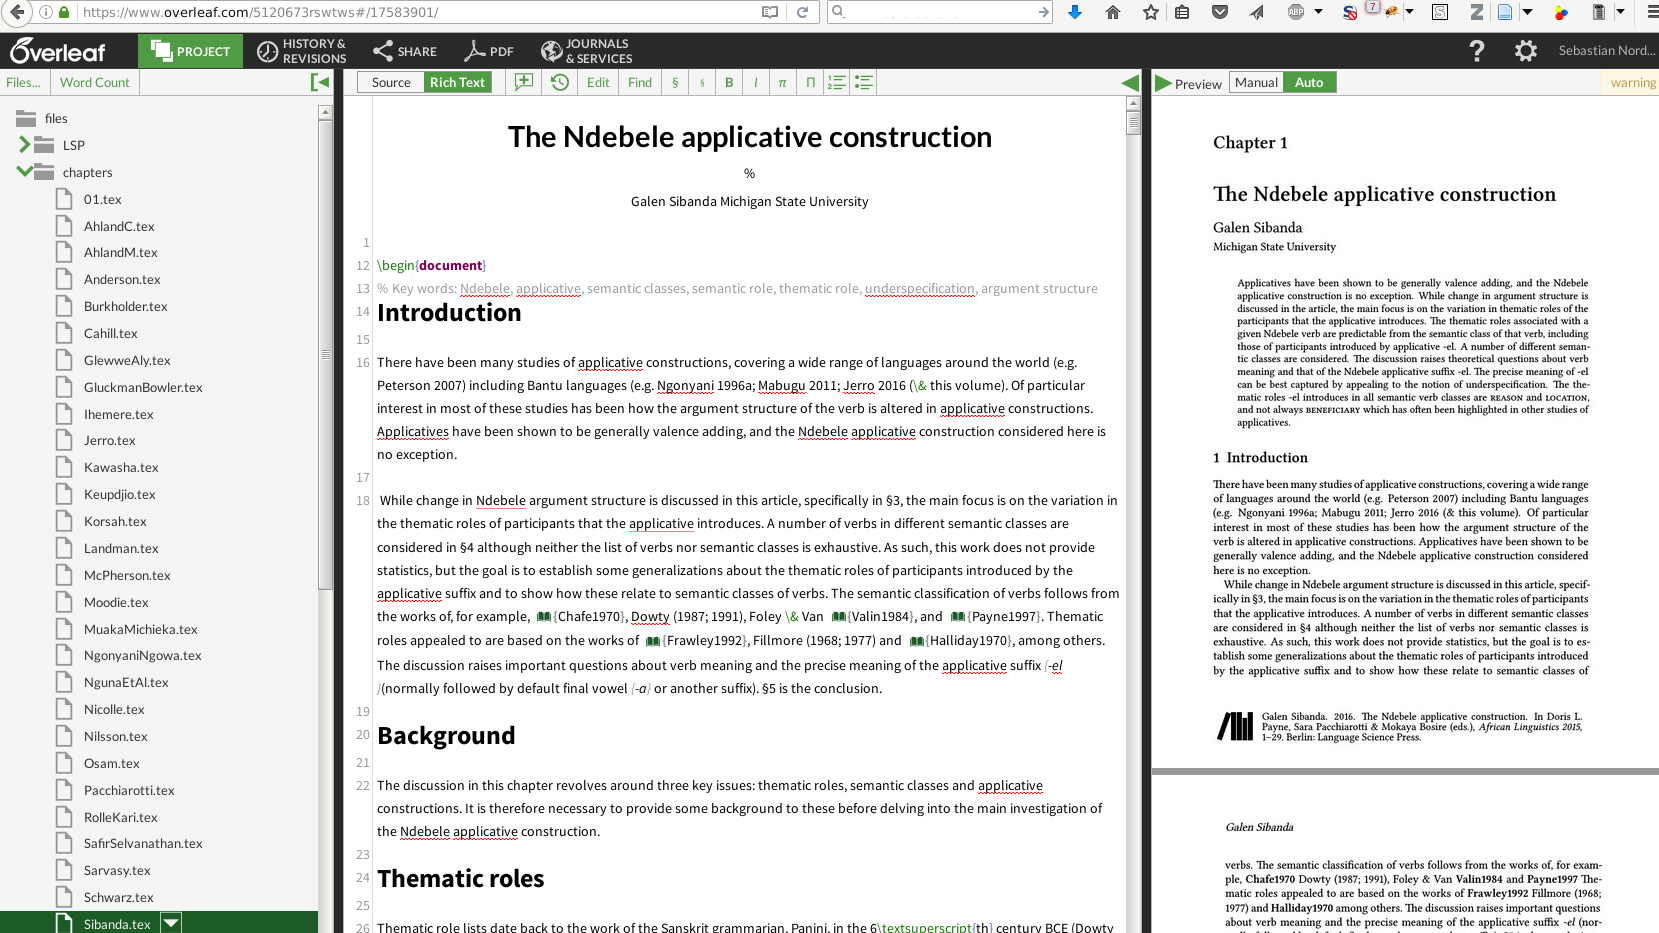
\includegraphics[width=\textwidth]{overleaf.png}
  \caption{Overleaf}
  \label{fig:latex:overleaf}
\end{figure}


\section{The skeleton}
The skeleton has a main file, which is called \verb+main.tex+. 
That main file draws information from a number of other files which are in the same directory. All those files start with \verb+local...+. Furthermore, the main file includes the chapters, which are found in the directory \verb+chapters/+.

\begin{table}[htb]
  \caption{File structure of the skeleton}
  \label{tab:latex:skeleton}
  \begin{tabularx}{\textwidth}{Xp{6cm}}
    \lsptoprule
    file & content \\
    \midrule
    \verb+localmetadata.tex+ & information about the author, the title, the ISBN, etc. \\
    \verb+localpackages.tex+ & extra packages you might require, for instance for syntactic trees or Hebrew text\\
    \verb+localcommands.tex+ & extra commands you might want to define, e.\,g.\ for very frequent abbrevations in your text\\
    \verb+localhyphenation.tex+ & for words where the \latex hyphenation algorithm does not produce the desired result      \\
    \verb+localbibliography.bib+ & your bibliography in \bibtex-format \\
    \verb+chapters/chapter1.tex+ & text \\
    \verb+chapters/chapter2.tex+ & text \\
... & text \\
    \verb+localseealso.tex+ & cross-references for the index  \\
    \lspbottomrule
  \end{tabularx}
\end{table}

A number of auxiliary files are generated on the fly, these are  \verb+.toc+ for the table of contents; \verb+.bbl+ for the bibliography; and \verb+.ind+, \verb+.and+, and \verb+.lnd+ for the indexes.  

\section{Using the \texttt{langsci} class}
There are a variety of programs for making writing \latex documents easier.

% For Microsoft Windows, Texniccenter is the most popular one (\figref{fig:latex:texniccenter}).
For Mac, Texshop (\figref{fig:latex:texshop}) and Texstudio (\figref{fig:latex:texstudio}) are popular choices.
For Linux, Kile is a very good \latex editor (\figref{fig:latex:kile}).

% \begin{figure}
% 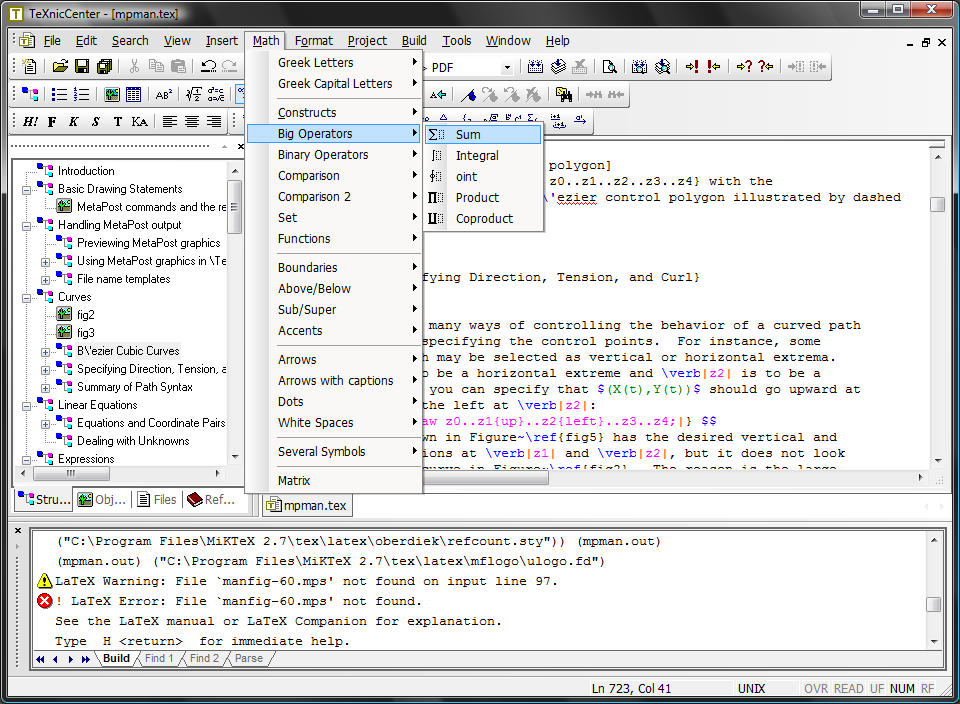
\includegraphics[height=.4\textheight]{texniccenter.png}
% \caption{Texniccenter}
% \label{fig:latex:texniccenter} 
% \end{figure}


\begin{figure}
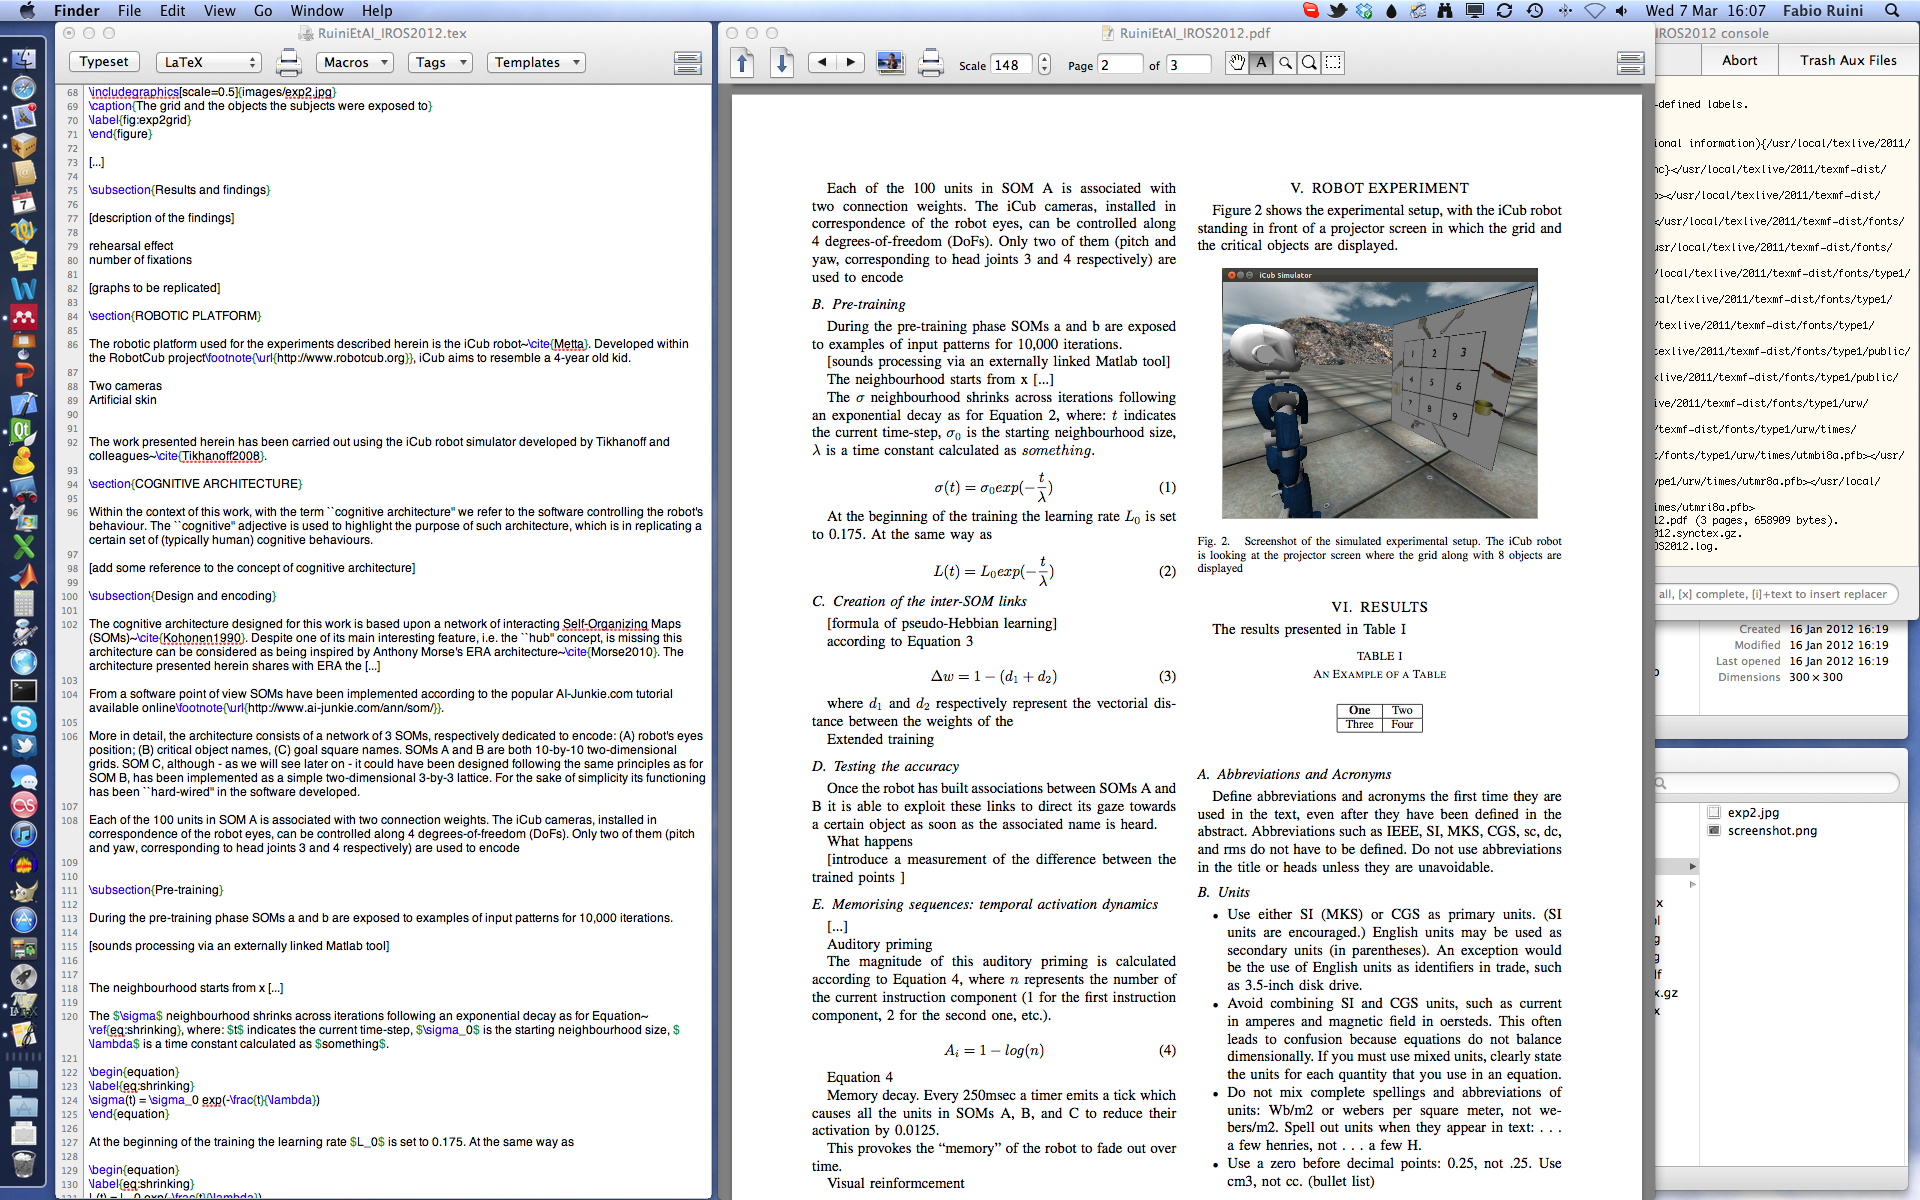
\includegraphics[height=.4\textheight]{texshop.png}
\caption{Texshop}
\label{fig:latex:texshop} 
\end{figure}

\begin{figure}
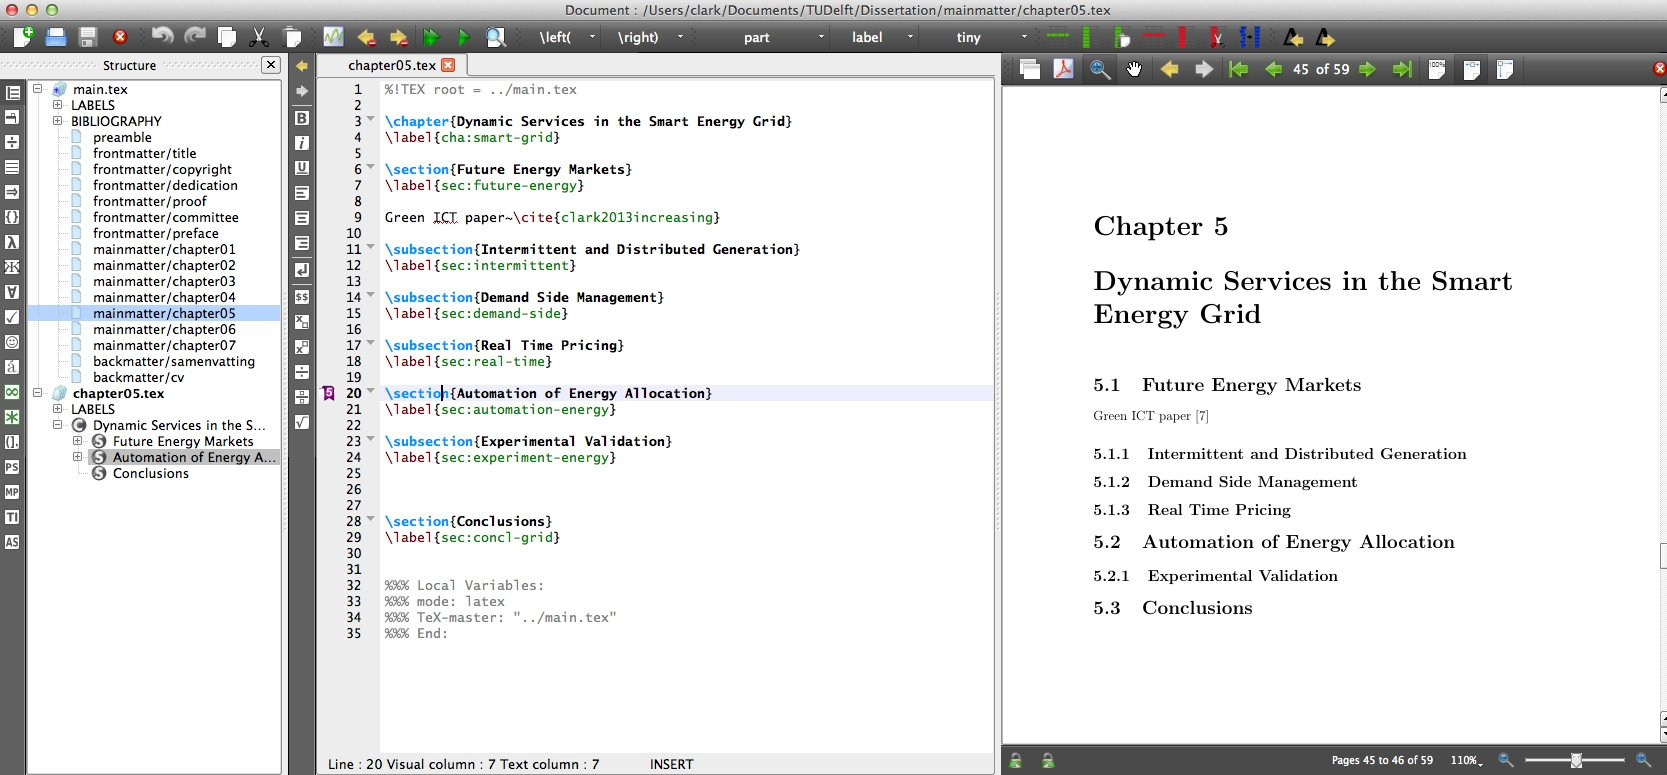
\includegraphics[width=\textwidth]{texstudio.jpg}
\caption{Texstudio}
\label{fig:latex:texstudio} 
\end{figure}


\begin{figure}
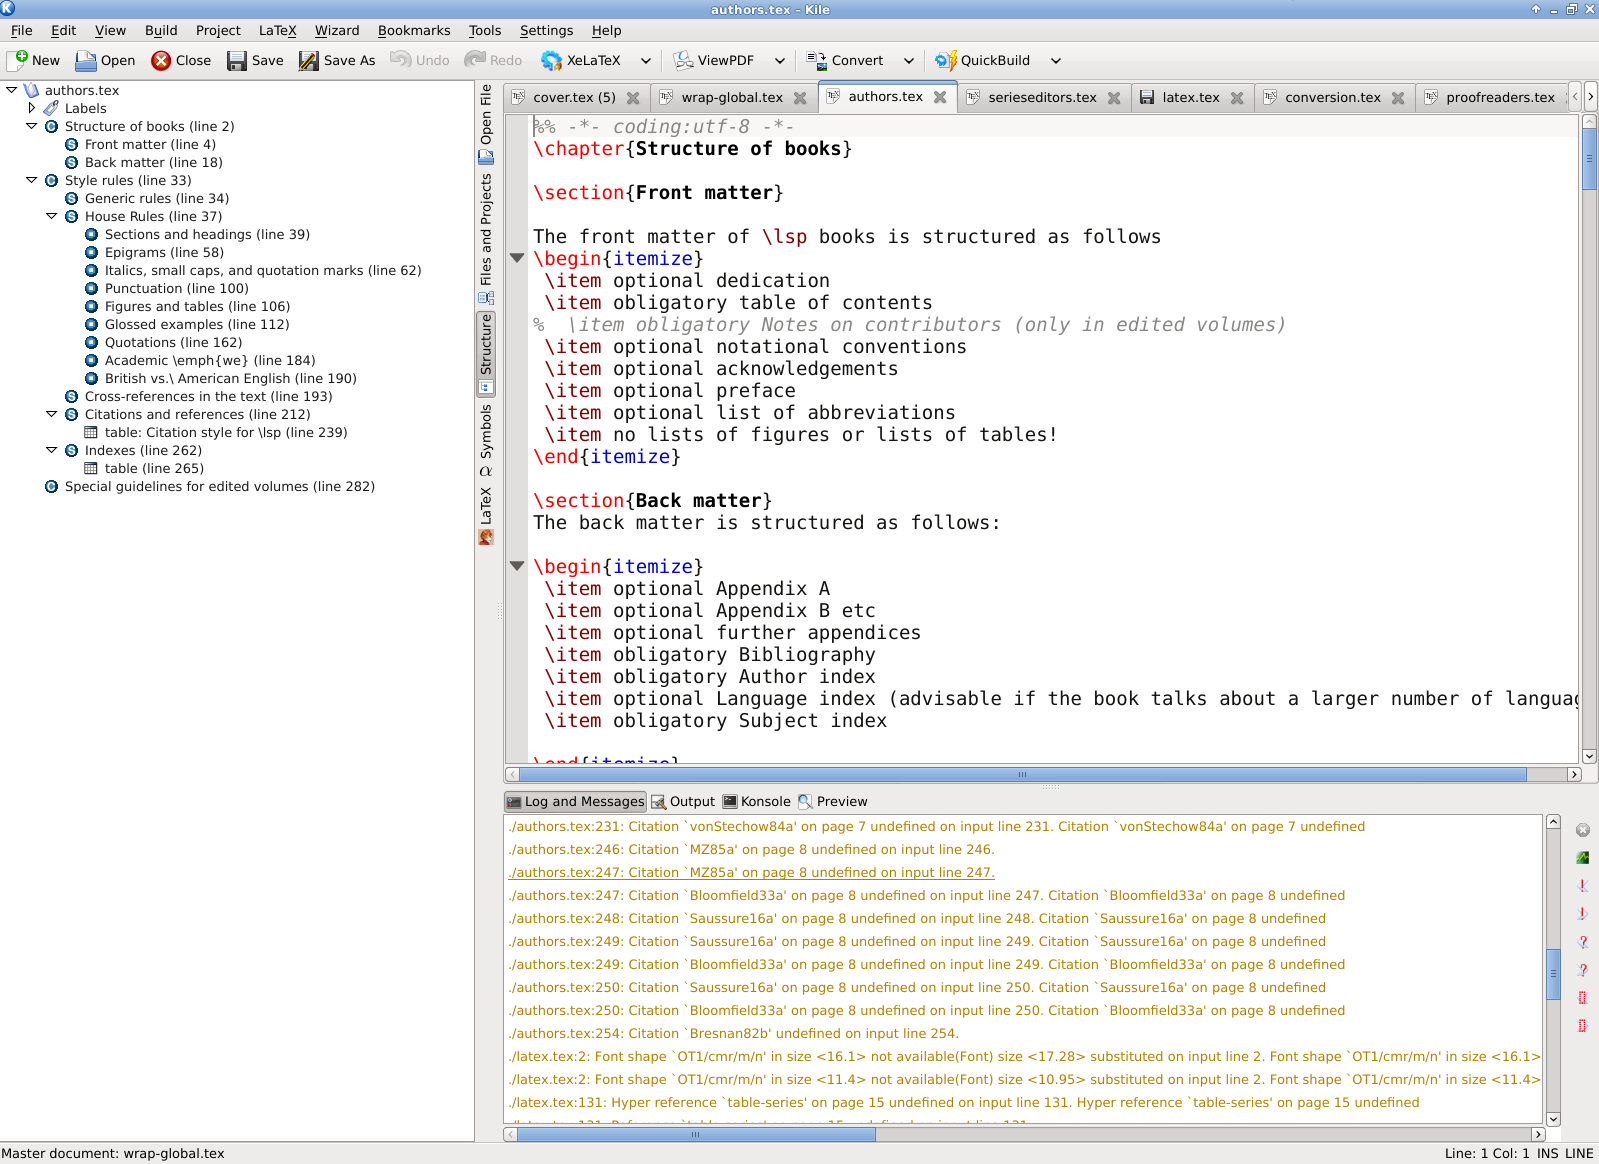
\includegraphics[width=\textwidth]{kile.png}
\caption{Kile}
\label{fig:latex:kile} 
\end{figure}

  
% \subsection{Included packages}
% The following packages are already loaded by default: 
% \verb+amssymb+, 
% \verb+authorindex+, 
% \verb+biblatex+, 
% \verb+booktabs+, 
% \verb+chngcntr+, 
% \verb+chngcntr+, 
% \verb+datetime+, 
% \verb+epigraph+, 
% \verb+etex+, 
% \verb+floatrow+, 
% \verb+fontspec+, 
% \verb+geometry+, 
% \verb+graphicx+, 
% \verb+hyperref +, 
% \verb+ifxetex+, 
% \verb+index+, 
% \verb+microtype+, 
% \verb+natbib+, 
% \verb+newtxmath+, 
% \verb+pbox+, 
% \verb+pst-barcode +, 
% \verb+rotating+, 
% \verb+scrpage2+, 
% \verb+showidx+, 
% \verb+textpos+, 
% \verb+tocstyle+, 
% \verb+url+, 
% \verb+xcolor+, 
% \verb+xspace+, 
% \verb+xstring+. 
% 
\section{Producing the document}
For an introduction to producing documents with \latex, see our screencast at \url{http://langsci-press.org/forAuthors}.
In your \latex editor, there are various ways to create a pdf from your sourcecode. Choose \verb+xelatex+. The first time you run it, it will produce a pdf with all the text, but with no table of contents. When you run it again, you will see the table of contents and the text. There are chances that your editor will show error messages. Common causes are unmatched braces or \verb+\begin{...}+ not followed by \verb+\end{...}+. See \url{https://github.com/langsci/latex/wiki/Troubeshooting} for a list of common errors and remedies.



In order to include the bibliography, you have to run \verb+bibtex+ to read the bibliography, and then again \verb+xelatex+ to include it into your document. Pay attention to error messages and warnings.
 
If you are using the skeleton for edited volumes, you have to run  \verb+bibtex+ on all \verb+*-blx.aux+-files (one for each chapter). If this is too cumbersome, you can also use the program \verb+bibtexvolume.sh+, which will do this for you and which is found in the skeleton as well. 

The creation of the indexes is a bit more complicated. You can leave this to the \lsp people. The relevant commands are:

\begin{verbatim}
makeindex -o lsp-skeleton.and lsp-skeleton.adx
makeindex -o lsp-skeleton.lnd lsp-skeleton.ldx 
makeindex -o lsp-skeleton.snd lsp-skeleton.sdx
\end{verbatim} 


\section{Adapting the structure of the document}
The general structure of the document is given by \lsp. You have a couple of options to change the structure:
\begin{itemize}
 \item You can choose the skeleton for monograph or edited volume
 \item You can add additional chapters to the directory \verb+chapters+, for instance\\ \verb+chapters/chapter4.tex+ or \verb+chapters/introduction.tex+. Make sure to add \verb+\chapter{Introduction}
This document describes how to create a manuscript with Language Science Press. It discusses what authors, volume editors and the auxiliary roles of proofreaders, typesetters and indexers have to know in order to produce high quality books.
+ (without \verb+.tex+) to your main file.
 \item You can add a preface, acknowledgements, or a list of abbreviations by removing the \verb+%+ from the relevant line in \verb+main.tex+.
 \end{itemize}



\section{Common commands}\label{sec:latex:commoncommands}
The wealth of commands available in \latex can be daunting at first sight. However, very soon you will see that you can get a very long way with some very basic commands. The first batch involve the structure of your document, i.e. the various levels of headings. These are:
\begin{itemize}
\item \verb+\chapter{titleofheading}+
\item \verb+\section{titleofheading}+
\item \verb+\subsection{titleofheading}+
\item \verb+\subsubsection{titleofheading}+
\end{itemize}

These commands give you a numbered title in the right layout.
%  For prefaces, acknowledgements, etc., which are not numbered, use \verb+\addchap{Preface}+ instead of \verb+\chapter{Preface}+. 
Other common commands are 
\verb+\label{labelname}+ 
to assign a label, and 
\verb+\ref{labelname}+
to refer to a label. It is good practice to use 
\verb+\sectref{labelname}+,
\verb+\tabref{labelname}+,
\verb+\figref{labelname}+,
to refer to sections, tables, and figures, respectively. A reference to this section will be \verb+see \sectref{sec:latex:commoncommands}+, which will produce ``see \sectref{sec:latex:commoncommands}''.

Other commands very often used in academic texts are \verb+\citet{somework}+ and \verb+\citep{somework}+. Use the former to cite a work in the running text and the latter to cite it in parentheses. In order to avoid double parentheses, you can use  \verb+\citealt{somework}+. Page numbers are added with \verb+\citet[99--123]{somework}+. Make sure to use a double hyphen for ranges, which will give a dash in the pdf. Citations work with keys from your \bibtex file. In the examples above \verb+somework+ is the key of a record in your \bibtex file. When \verb+somework+ is cited in the document, the pdf will show the right citation in the right style, and the work will be added automatically to the list of references at the very end. Please refer to the guidelines for bibliographies for more information.


If some text should not be in the normal font, use 
\verb+\textit{text to change}+ for italics, 
\verb+\textbf{text to change}+ for boldface, 
\verb+\textsc{text to change}+ for small capitals. Boldface must not be used in running text. It may be used for emphasis in linguistic examples. 
There is generally no need to use underlining. If you want to use underlining, get in touch with support.

\subsection{Linguistic examples}
Linguistic examples are typeset like this

\begin{verbatim}
\ea\label{ex:examplelabel}
\langinfo{French}{Indo-European}{personal knowledge}\\
\gll  Jean aim-e                    Marie \\
      John love-\textsc{3s.pres.ind} Mary \\
\glt `John loves Mary.'    
\z
\end{verbatim}

\newcommand{\sg}{\textsc{sg}}
\newcommand{\prs}{\textsc{prs}}
\newcommand{\ind}{\textsc{ind}}
This gives you
% \todo{fix index}
\ea\label{ex:examplelabel}
\langinfo{French}{Indo-European}{personal knowledge}\\
\gll  Jean aim-e Marie \\
      John love-{3\sg.\prs.\ind} Mary \\
\glt `John loves Mary.'    
\z

Rough alignment of glosses in the source text can be helpful, but is not necessary. \latex will take care of alignment of the glosses automatically. 
% Most glosses from the Leipzig Glossing Rules can be accessed via shortcuts. The example above could also be typeset as
% 
% \begin{verbatim}
% \ea\label{ex:examplelabel}
% \langinfo{French}{Indo-European}{personal knowledge}\\
% \gll  Jean aim-e                 Marie \\
%       John love-{3\sg.\prs.\ind} Mary \\
% \glt `John loves Mary.'    
% \z
% \end{verbatim}

For more complicated examples with more lines, judgments, additional information and the like, refer to the showcases section, or to the documentation of the package \verb+langsci-gb4e+.
\verb+\langinfo+ should be used if the language cannot be assumed to be widely known. The first argument is the language, the second the family, the third the source. If the family is left blank, it will not display. If you give a reference in the source, use \verb+\citealt+ rather than \verb+\citep+.

To avoid a page break in an example, put it between \verb+\protectedex{...}+. 

\begin{verbatim}
\protectedex{
\ea\label{ex:examplelabel}
\langinfo{French}{Indo-European}{personal knowledge}\\
\gll  Jean aim-e                 Marie \\
      John love-{3\sg.\prs.\ind} Mary \\
\glt `John loves Mary.'    
\z
}
\end{verbatim}
 
\subsection{Graphics}
In order to add a graphics file, use the following stretch of code

\begin{verbatim}
\begin{figure}
  \includegraphics[height=.3\textheight]{figures/filename.png}
  \caption{Some good caption.}
  \label{fig:chapterhandle:keytofigure}
\end{figure}
\end{verbatim}

You can adapt the height, or use \verb+\textwidth+ instead of \verb+\textheight+.

\subsection{Tables}
\subsubsection{Basic tables}
In order to add a table, use the following stretch of code:

\begin{verbatim}
\begin{table} 
  \begin{tabularx}{\textwidth}{XXX}
    \lsptoprule
    German  & French  & Spanish \\
    \midrule
    Zelle   & cellule & celda    \\
    Zelle   & cellule & celda    \\
    Zelle   & cellule & celda    \\
    \lspbottomrule
  \end{tabularx}
  \caption{Some good caption.}
  \label{tab:chapterhandle:keytotable}
\end{table}
\end{verbatim}

This will give you  \tabref{tab:chapterhandle:keytotable}. There are ways to add additional vertical lines, but this should generally not be done. 

\begin{table}[h]
  \begin{tabularx}{\textwidth}{XXX}
    \lsptoprule
    German  & French  & Spanish \\
    \midrule
    Zelle   & cellule & celda    \\
    Zelle   & cellule & celda    \\
    Zelle   & cellule & celda    \\
    \lspbottomrule
  \end{tabularx}
  \caption{Some good caption.}
  \label{tab:chapterhandle:keytotable}
\end{table}

You can use \verb+\tablevspace+ for separation of groups within a table. 

You should not assume that a figure or table will be placed exactly where it appears in the text. Therefore, references like ``in the table above/below'' should not be used. 

You can adapt the width of the table by using \verb+.75\textwidth+,  \verb+.66\textwidth+, or \verb+.5\textwidth+.

\verb+XXX+ tells \latex to split the available space into three equal portions and to justify the content inside the cells. 

\subsubsection{Tweaking tables}
In order to give explicit width, use \verb+p{1.75cm}+ or whatever the desired length might be, instead of \verb+X+. 
This will set the column width to 1.75cm and justify the cell contents. If you would rather have left-aligned content without hyphenation, use \verb+L{1.75cm}+, for center use \verb+C{1.75cm}+, for right-aligned use \verb+R{1.75cm}+.

If you want columns of equal width, use \verb+X+ as above for justified, \verb+Q+ for left-aligned, \verb+S+ for right aligned and \verb+Z+ for centered.

If you want the cell to be exactly the width of its content, use \verb+l+, \verb+r+, \verb+c+, respectively. You can mix all column types freely as in \tabref{tab:colmixes}. In case you find this to complex, stick to \verb+l+ and \verb+X+ for a start.

\begin{table}
 \begin{tabularx}{\textwidth}{lXrR{2cm}Qc}
\lsptoprule
l & X & r & R\{2cm\} & Q & c \\
\midrule
  start & long cell w/   wrapping words & .95 & This content is very long but does not hyphenate. It is right-aligned. The cell has a width of 2cm. & This cell, together with cells in column 2, takes up all remaining space, shared equally. It does not hyphenate. & center\\
s & & .0001 & &&  c \\ 
\lspbottomrule
\end{tabularx} 
\caption{Illlustration of different column types.}
\label{tab:colmixes}
\end{table}


\subsection{Footnotes}
In order to add footnotes, use the command \verb+\footnote{...}+. If you want to use a footnote in an example, use \verb+word {\footnotemark} word word+ and add a line with \verb+\footnotetext{text of the footnote}+ just before the translation of the example. You should not add footnotes to tables or figures. Add the content in the running text, either in the main body of the text or as a footnote. 

\subsection{Landscape}

A common requirement is to put pages in landscape orientation rather than portrait. In order to do this, use \verb+sidewaysfigure+ or \verb+sidewaystable+ instead of the normal \verb+figure+ or \verb+table+.

\subsection{Fitting large content on the page}
Another common requirement is fitting a table or other element which is a bit too large on the page. In order to do this, use \verb+\fittable{stuff to resize}+. This works for figures as well. 

For other special needs, please contact our coordinator at \url{support@langsci-press.org}. 

\subsection{Computer code}
Please use the \verb+listings+ environment. You can change which words should count as keywords.

\begin{verbatim}
\begin{lstlisting}[language=Python, stringstyle=\color{blue}]
 greeting = "Hello"
 addressees = ["World", "Sky"]
 for addressee in addresses:
    print greeting, addressee
\end{lstlisting}
\end{verbatim}
 
\begin{lstlisting}[language=Python, stringstyle=\color{blue}]
 greeting = "Hello"
 addressees = ["World", "Sky"]
 for addressee in addresses:
    print greeting, addressee
\end{lstlisting}

\section{Adapting the class to your needs}

Additional packages can be added via \verb+\usepackage{packagename}+ in the file \verb+localpackages.tex+.
Addtional commands can be added via \verb+\newcommand{\commandname}{commanddefinition}+ in the file \verb+localcommands.tex+. 


Different subdisciplines of linguistics have different requirements. Syntactic trees, generously stacked diacritics, attribute-value matrices, foreign scripts (possibly right-to-left) or OT-tableaus come to mind. Have a look at the ``showcases'' guideline to see how to typeset these elements.


 
   
\section{Drafts}

Since \lsp does not have any commercial interest, you can put your book on webpages and distribute it
freely. We encourage authors to do this in order to discuss the work and improve it before final
publication. If authors want to circulate prefinal versions, they can use the option
\texttt{draftmode}. This prints a large watermark onto the first page and adds a footer to ever page
that informs the reader about the fact that they are reading a draft and the date and time of the
creation of the draft.
  

\chapter{Conversion} 
\section{Conversion using the webservice}
While it is preferable to work in {\latex} from the start, this is not always possible. For edited volumes, for instance, it is common that not all authors can acquire the necessary skills in due course. For those cases, you can use the templates for MS Word and LibreOffice provided on \url{http://langsci-press.org/templatesAndTools}. Follow the instructions in the templates. When you are finished, upload your file to \url{http://glottotopia.org/doc2tex/doc2tex}. This will give you a file which you can copy into the skeleton (\figref{fig:conversion:glottotopia}). You have the choice between ``raw'' and ``mod''. Generally,  ``mod'' is preferable as a number of adaptations for linguists and \lsp are already in place. If you run into problems with ``mod'', you can use  ``raw'' as a fallback. You can then either copy and paste the converted document to a file of your own, or you can open the document directly in Overleaf (\figref{fig:conversion:overleaf}).

Note that the converter was built in 2015. Newer versions of MS Word/LibreOffice may introduce items unknown to the converter. In this case, contact support immediately.

\begin{figure}
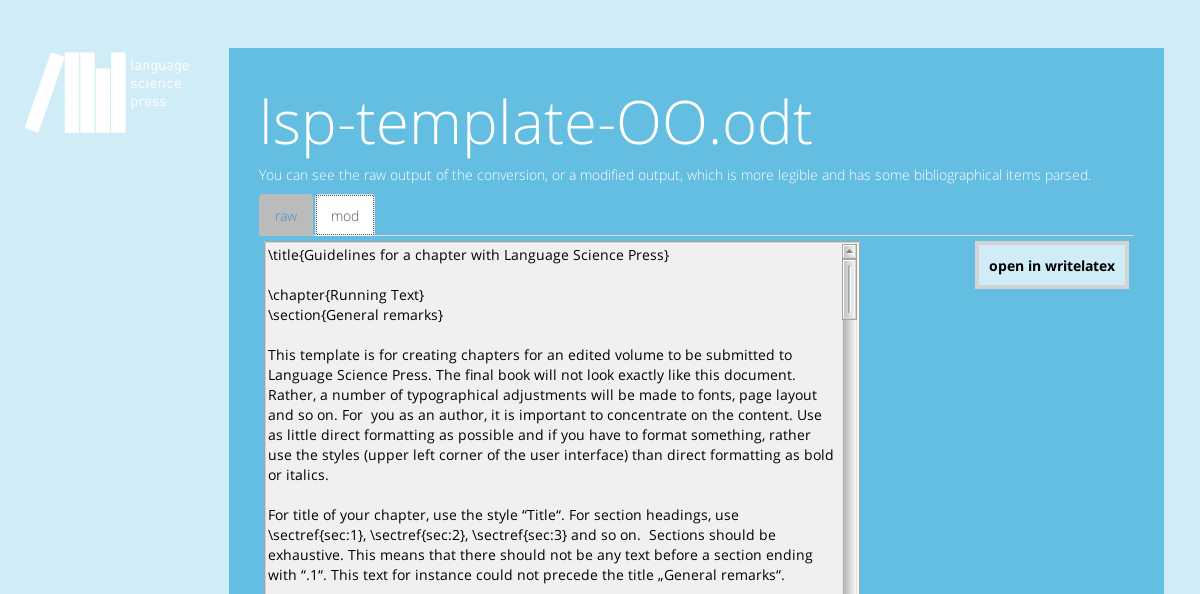
\includegraphics[width=\textwidth]{converter.png} 
\caption{After converting the template on \url{http://glottotopia.org/doc2tex/doc2tex}.}
\label{fig:conversion:glottotopia}
\end{figure}

\begin{figure}
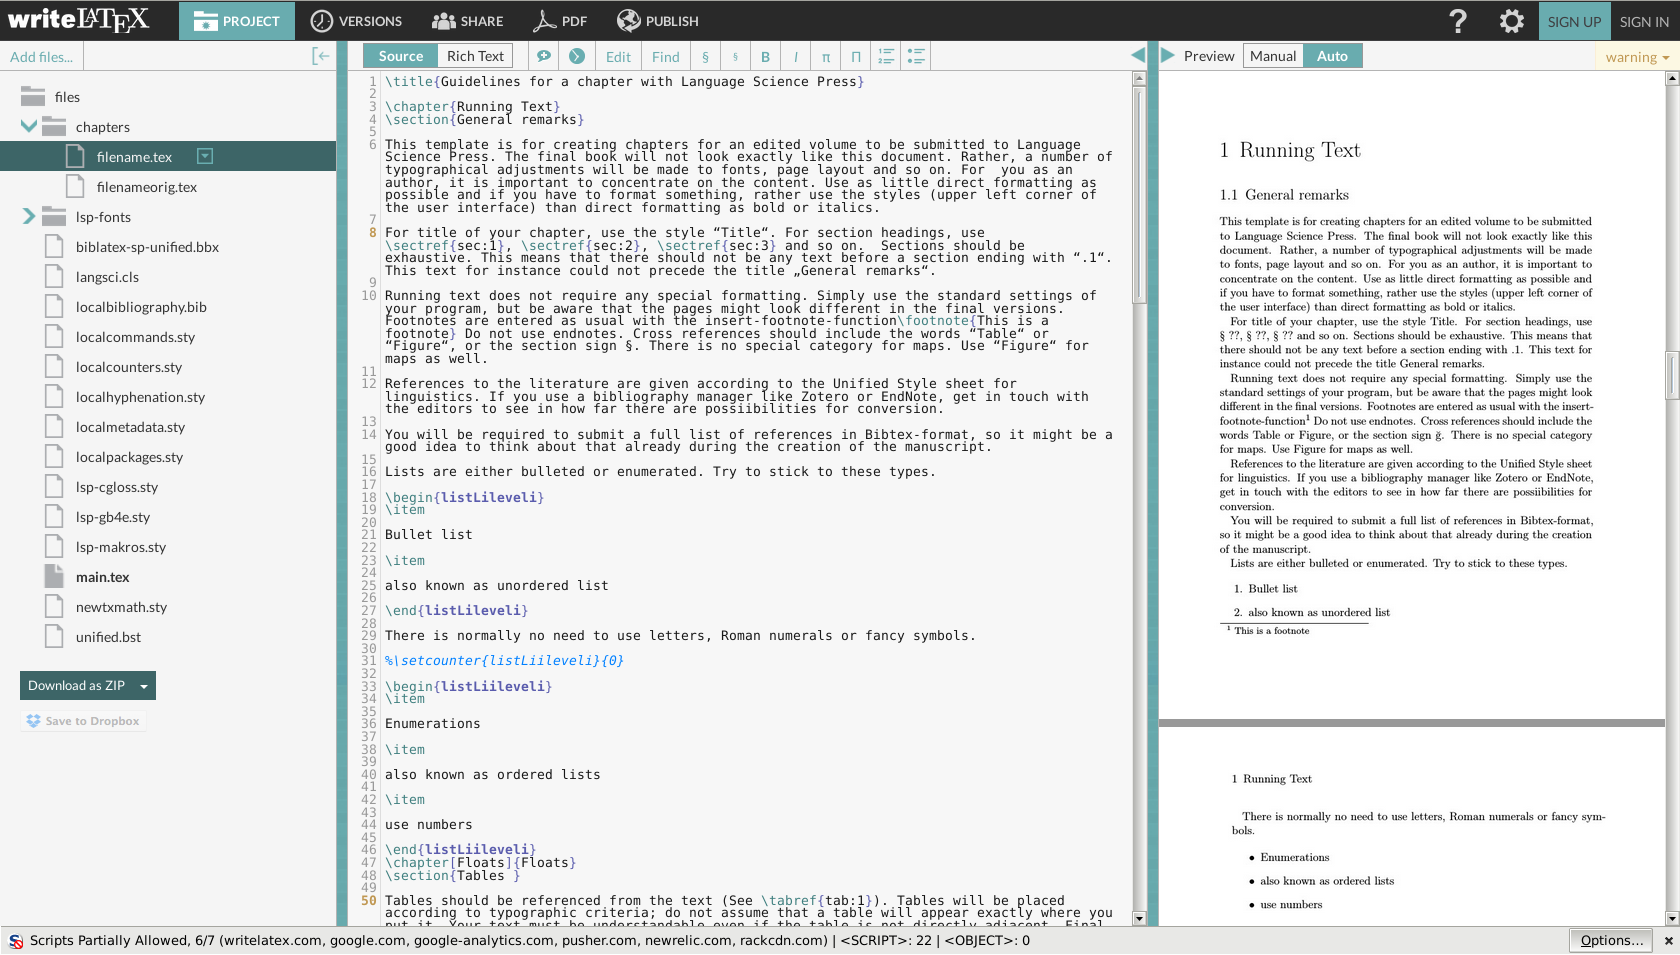
\includegraphics[width=\textwidth]{conversionwritelatex.png} 
\caption{Opening the converted document on Overleaf.}
\label{fig:conversion:overleaf}
\end{figure}

\section{Manual conversion}
If you want to convert your file on your local computer, you can use the program \verb+writer2latex+. The relevant command is 
\begin{verbatim}
w2l -wrap_lines_after=0 -multilingual=false 
-simple_table_limit=10 -use_supertabular=false 
-float_tables=true -float_figures=true 
-use_caption=true -image_options=width=\textwidth 
-inputencoding=utf8 -use_tipa=false -use_bibtex=true  
-formatting=convert_most -ignore_empty_paragraphs=true 
-use_color=false -page_formatting=ignore_all
 -use_hyperref=true mydocument.odt
\end{verbatim}

\section{Manual postprocessing}
While the converter tries to convert as much as possible, there are a some places where manual postprocessing is still required.
These include graphics, cross-references and some bibliographical references.

% \subsection{Examples}
% The output of automatically converted examples has the example formatting separated from the example content.  
% \begin{verbatim}
% \ea%1
%   \label{ex:1}
%   \langinfo{lg}{fam}{src}\\
%   \gll\\
%       \\
%   \glt
% \z
% 
% Ceci n' est pas une pomme
% 
%  this \textsc{neg}  {\cop.3\sg.\prs} \textsc{neg}   
% \textsc{det.f} apple
% 
% ``This is not an apple''
% \end{verbatim}
% 
% One has to manually join the former and the latter part to get
% 
% \begin{verbatim}
% \ea%1
%   \label{ex:1}
%     \langinfo{lg}{fam}{src}\\
%   \gll Ceci n'             est                 pas une pomme \\
%       this \textsc{neg} {\cop.3\sg.\prs} \textsc{neg}   
%       \textsc{det.f} apple\\
%   \glt ``This is not an apple''
% \z 
% \end{verbatim} 
% 
% Furthermore, \verb+\langinfo+ has to be adapted to reflect the correct language, family and source of the example, or removed altogether. In this case, one would use  \verb+\langinfo{French}{Indo-European}{René Magritte}\\+

\subsection{Graphics}
All graphics are commented out by default since the files will not be available on Overleaf until you upload them. So the following stretch

\begin{verbatim}
 \begin{figure}[h]
[Warning: Image ignored] %Unhandled or unsupported graphics:
%\includegraphics[width=\textwidth]
{a8dc5773011814b3b98013db7af4ec7e9-img1.png}
\caption[Some caption]{Some caption}
\end{figure}
\end{verbatim}

has to become


\begin{verbatim}
\begin{figure}
 \includegraphics[width=\textwidth]{figures/realnameofthefile.png}
 \caption{Some caption}
 \label{fig:chaptername:filehandle}
\end{figure}
\end{verbatim}

\subsection{Cross-references}
Generally, references to sections and examples should work. Occasionally, there might be problems with stretches like ``(12a)'' or ``(12-15)''. These have to be fixed manually.

\subsection{Bibliographical references}
The most common bibliographical references should work. Where authors have names which consist of two parts (such as ``Van Valin''), the author is often misrecognized as ``Valin''. Also, stretches like ``Smith 2000, 2001a,b, 2002'' will need manual postprocessing. 





proofreaders


\chapter{Indexing}
\lsp books have an obligatory Name Index and an obligatory Subject Index. The Language Index is optional and should be used if your work makes reference to more than one language. 
For the various ways to add entries to the index, refer to \tabref{tab:latex:indexentriese}. For every index, there are two commands. The shorter one adds a term to the relevant index but does not change your text. This is useful if the term you want to add to your index does not appear in exactly the same way in the text. If the term is indeed identical, you can use the command with an extra \computer{i}.

\begin{table}[h]
\caption{Commands for creating index entries.}
\label{tab:latex:indexentriese}
 \begin{tabular}{p{2.5cm}>{\tt\small\raggedright}p{6.5cm}p{3cm}}
  \lsptoprule
  type & \rm\normalsize command & indexed term \\
  \midrule
  Subject Index& Nominalized sentences \textbf{$\setminus$is\{nominalization\}} are current. & nomina\-lization \\
  \mbox{Subject Index} identical& ... while \textbf{$\setminus$isi\{nominalization\}} is less frequent ...  & nomina\-lization \\[2em]
  Language Index & Varieties of Chinese \textbf{$\setminus$il\{Sinitic languages\}} differ in that ...& Sinitic languages \\
  Language Index identical& The \textbf{$\setminus$ili\{Sinitic languages\}}, \mbox{however}, ... & Sinitic languages \\[2em]
  Author Index & In Homeric \textbf{$\setminus$ia\{Homer\}} language, ...  & Homer\\
  \mbox{Author Index} identical & This contradicts \textbf{$\setminus$iai\{Homer\}}, who had advocated ... & Homer \\
  \lspbottomrule
 \end{tabular}
\end{table}

If there are two or more entries on subsequent pages, the index generation will automatically produce a range. So, instead of `33,34,35,36', it will print out `33--36'. You can produce ranges yourself by using \computer{{\bs}is\{someterm|(\}} for the start and  \computer{{\bs}is\{someterm|)\}} for the end of the range. 

Do not use the indexing commands directly before punctuation as it can produce unwanted white space. Put it after the punctuation instead.

If you compile your document with the option \computer{draftmode} all indexed terms will show up in the margins.

When your are done with adding index terms to your document, the following commands will produce the Subject Index and the Language Index
\begin{verbatim}
makeindex -o yourfilename.ind yourfilename.idx
makeindex -o yourfilename.lnd yourfilename.ldx
\end{verbatim}
 
The author index should be produced automatically.
% \begin{verbatim} 
% authorindex -i -p yourfilename.aux > yourfilename.bib.adx
% sed 's/|hyperpage//' yourfilename.adx > yourfilename.txt.adx 
% cat yourfilename.bib.adx yourfilename.txt.adx > yourfilename.combined.adx
% makeindex -o yourfilename.and yourfilename.combined.adx
% \end{verbatim}

After the creation of the indexes, check for every index whether it contains only terms that should be found in this index (no languages in Subject Index and vice versa). Furthermore, check that every concept has exactly one entry in the index. It is easy to index the same concept once in the singular and then again in the plural, or once with a hyphen and once without. 

For the Name Index, make sure that every author has exactly one entry. Common errors include abbreviated names, middle initials which are present in one entry but absent in another, different transcriptions of a name, and diacritics. These issues are fixed by opening your bibliography file and conforming the names of the authors there.

After your indexed terms are final, check the Name Index for terms which are not names. This happens if one of your cited works has an institution as the author. Open the \computer{.adx} file and remove that entry. Be aware that a recompilation of your index will overwrite your changes.

Check your index for overlong lines. Use hyphenations \computer{{\bs}mbox\{...\}} or \computer{{\bs}newline}s in the \computer{.adx} file to repair these. Again, a recompilation of the index will overwrite your changes.

typesetters

length of titles, page headers, toc entries

fit floats

place floats

overfull hboxes

full pages

clubs and widows

clubs and widows bibliography

 
\chapter{Commitment to openness}
\section{Open Access and its friends}
\lsp has a commitment to openness. This means that, beyond Open Access, we also use Open Source Software, and we make our workflows and organizational structure publicly available so that other projects can draw on our work. The licenses we use obey the \href{Open Definition}{http://opendefinition.org}, meaning that everybody is always free to use our work if they attribute it properly.




\section{Tracking progress}
\subsection{github}
A book is a complex document. Once your book is in final production mode, we use github to track versions and changes (\figref{fig:latex:github}). You can use github during the writing process as well (in fact, this will make the transition much smoother).

\subsection{Trello}
In order to keep things organized, we use Trello (\figref{fig:latex:trello}). Trello allows to distribute tasks such as bibliography update, proofreading, index creation and so on and keeps track of progress.

\begin{figure}
\caption{Github highlighting version history}
\label{fig:latex:github}
 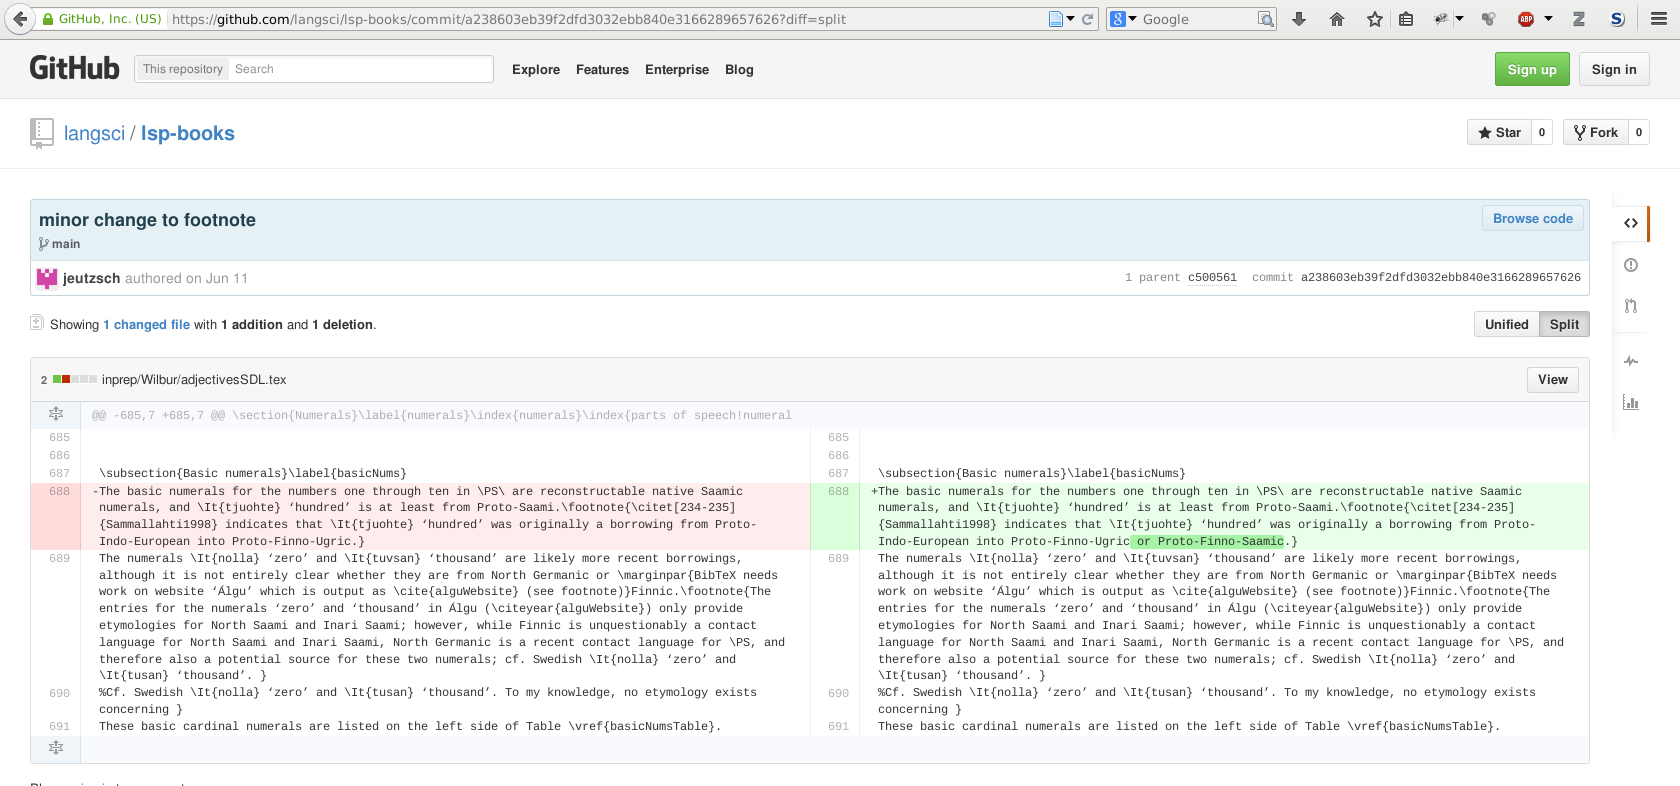
\includegraphics[width=\textwidth]{github.png}
\end{figure}

\begin{figure}
\caption{Trello}
\label{fig:latex:trello}
 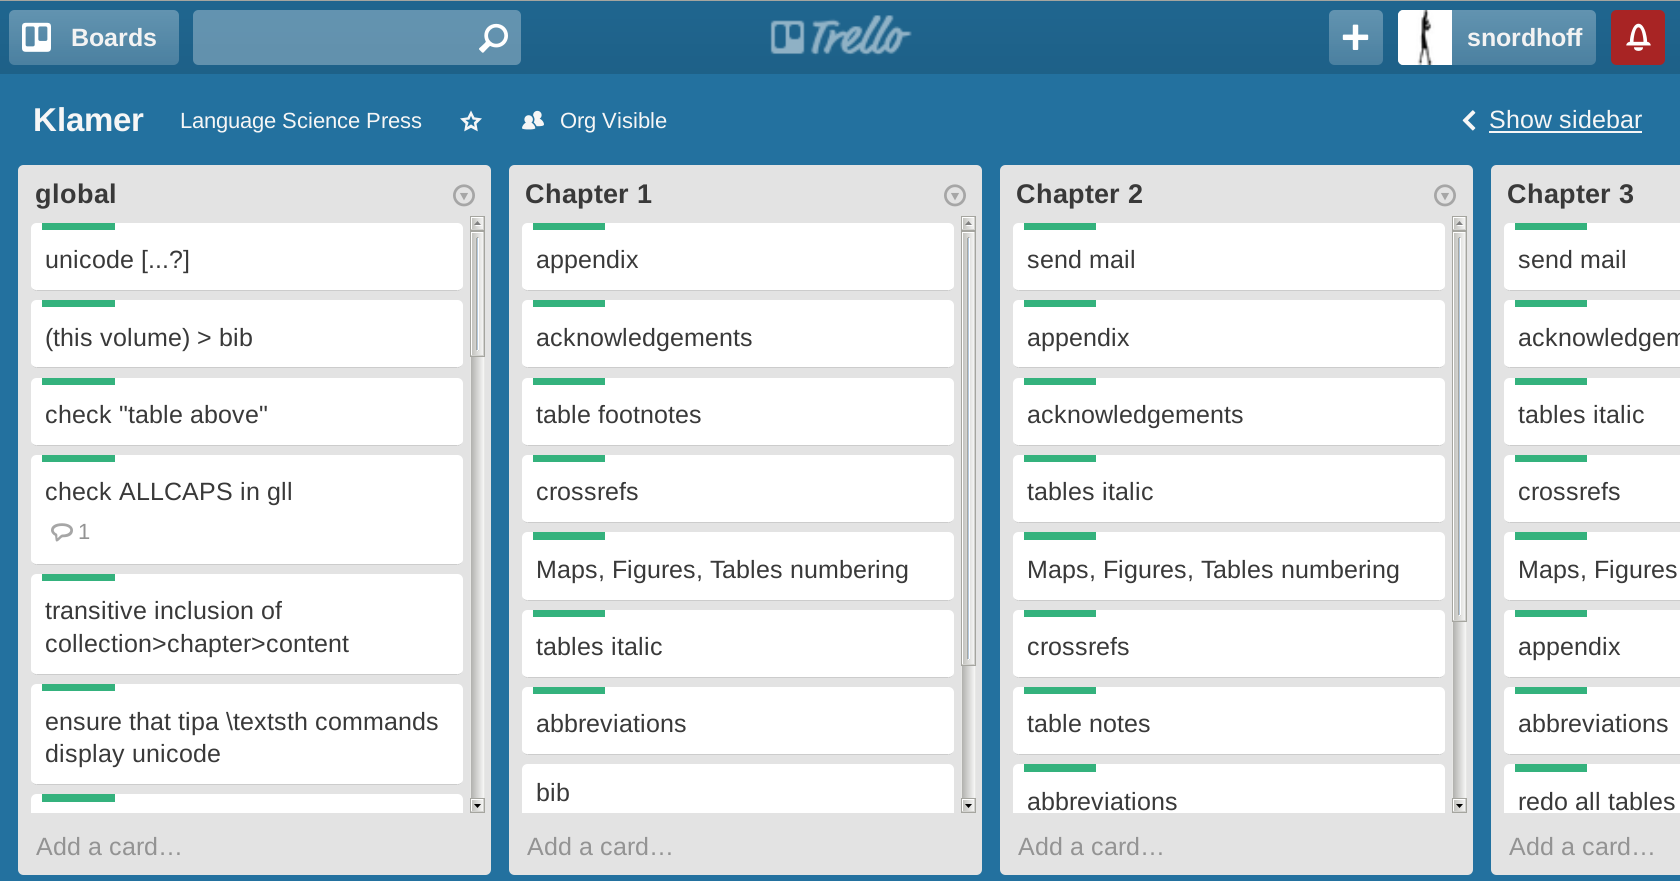
\includegraphics[width=\textwidth]{trello.png}
\end{figure}


\chapter{Showcases}

There is a huge amount of packages that can be used for various purposes. \citet{MG2013a} is a good
reference book. This section discusses some aspects of some packages that are relevant for
linguistics. Every \latex package comes with a documentation and users should consult these
documentations, too. The purpose of this section is to point users to the packages that we think
serve their purpose best and that are compatible with other packages and the \lsp classes, as this
book proves.

\section{Glossed examples}

Glossed\is{glossing|(}\ispackageb{lsp-gb4e} examples are typeset with a modified version of the \texttt{gb4e}\ispackage{gb4e} package by Craig
Thiersch\ia{Thiersch, Craig}. The modified package is called \texttt{lsp-gb4e}. 
% % It is contained in the styles directory that is delivered with the \lsp \latex classes. It differs from the original package in loading a version of \texttt{gloss} that was modified by Alexis Dimitriadis\ia{Alexis Dimitriadis} in order to be compatible with \texttt{jambox} (see Section~\ref{sec-jambox}).

Simple examples like \REF{ex:showcases:simple} can be typeset as shown below.
\ea\label{ex:showcases:simple}
\iw{Mann}\iw{schlafen}
\gll Der Mann schläft.\\
     the man  sleeps\\
\glt `The man sleeps.'
\z
\begin{verbatim}
\ea
\gll  Der Mann schläft.\\
      the man  sleeps\\
\glt `The man sleeps.'
\z
\end{verbatim}

Grammaticality judgments can be added in brackets. Note that in this case, braces have to be used around the rest of the example
\ea[*]{\label{ex:showcases:ungrammatical}
\iw{Mann}\iw{schlafen}
\gll Der Mann schlafen.\\
     the man  sleep\\
\glt `(The man sleeps.)'
}
\z
 
\newpage
\begin{verbatim}
\ea[*]{
  \gll  Der Mann schläft.\\
        the man  sleeps\\
  \glt `(The man sleeps.)'
  }
\z
\end{verbatim} 

Lists of examples can be typeset with nested \verb+\ea+  and \verb+\z+  respectively. The example in
\REF{ex:showcases:list} shows how the sentences can be aligned properly. Note that the first example in a list gets \verb+\ea+, the subsequent ones get \verb+\ex+. Also note the empty grammticality judgment for the first example in order to align it with the second example, which has a~*.


\ea  \label{ex:showcases:list}
\ea[]{
\iw{Linguist}\iw{Nobelpreis}\iw{glauben}
\gll Ich glaube dem Linguisten nicht, 
     einen Nobelpreis gewonnen zu haben.\\
     I believe the linguist not 
     a Nobel.prize won to have\\
\glt  `I don't believe linguist's claim 
      that he won a Nobel prize.'
}
\ex[*]{
\gll Dem Linguisten einen Nobelpreis  glaube  
     ich nicht gewonnen zu haben.\\
     the linguist   a     Nobel.price believe 
     I   not   won      to have\\
}
\z
\z  

\begin{verbatim}

\ea 
 \ea[]{
 \gll Ich glaube dem Linguisten nicht, 
     einen Nobelpreis gewonnen zu haben.\\
     I believe the linguist not 
     a Nobel.prize won to have\\
 \glt  `I don't believe linguist's claim 
      that he won a Nobel prize.'
}
\end{verbatim}
\newpage
\begin{verbatim}
 \ex[*]{
 \gll Dem Linguisten einen Nobelpreis  glaube  
      ich nicht gewonnen zu haben.\\
      the linguist   a     Nobel.price believe 
      I   not   won      to have\\
 }
 \z
\z
\end{verbatim}
 

If you want to add a footnote\is{footnote|(} that provides the source of an example as in \REF{ex:showcases:footnote}, you can do
this as follows:
\ea\label{ex:showcases:footnote}
\gll Piloten         fik frataget    sit certifikat\footnotemark\\
     pilot.\textsc{def} got deprived.of his license\\
\footnotetext{KorpusDK.}
\glt `The pilot was deprived of his license to fly.'
\z 
\begin{verbatim}
\ea
\gll Piloten fik frataget sit certifikat{\footnotemark}\\
     pilot.\textsc{def} got deprived.of his license\\
\footnotetext{KorpusDK.}
\glt `The pilot was deprived of his license to fly.'
\z 
\end{verbatim}
Please call the \verb+\footnotetext+ command before the translation, since otherwise the
footnotetext may be typeset on a page that is different from the one where the footnotemark is set.\is{footnote|)}

% For the typesetting of an additional line with the original script, one may use \verb+\glll+ rather
% than \verb+\gll+. \REF{ex:shown:chinese} shows a Chinese example:
% \ea
% \label{ex:shown:chinese}
% \glll 狗       叫     了。\\
%       gou3     jiao4   le\\
%       dog      bark    \textsc{asp/crs}\\
% \glt `The dog is barking.'/`The dogs are barking.'
% \z
% 
% \begin{verbatim}
% \ea
% \glll 狗       叫     了。\\
%       gou3     jiao4   le\\
%       dog      bark    \textsc{asp/crs}\\
% \glt `The dog is barking.'/`The dogs are barking.'
% \z
% \end{verbatim}

% You can use up to \verb+\glllllll+ if you need additional lines.

In some subdisciplines of linguistics (e.\,g.\ typology) the examples are written in italics as in the
following example:
\ea
\def\exfont{\normalsize\itshape}
\gll Piloten         fik frataget    sit certifikat{\footnotemark}\\
     pilot.{\scshape def} got deprived.of his license\\
\footnotetext{KorpusDK.}
\glt `The pilot was deprived of his license to fly.'
\z 
This is done automatically according to the series you publish in. 
% of course this is not true for the code above ... 

If the series decides to use italics, it has to be ensured that structural markup like brackets are not typeset in italics. Use \verb+\ob+ for opening brackets and \verb+\cb+ for closing brackets. \verb+\op+ and \verb+\cp+ provide the same for parens.
\begin{verbatim}
\ea
\gll ein {\ob}interessantes  Beispiel{\cb}\\
     an   interesting        example\\
\glt `an interesting example'
\z 
\end{verbatim}
\ea
\def\exfont{\normalsize\itshape}
\gll ein {\ob}interessantes       Beispiel{\cb}\\
     an   interesting example\\
\glt `an interesting example'
\z 
\is{glossing|)}\ispackagee{lsp-gb4e}

In order to align the gloss with the beginning of the source word, and not with the bracket, you can use \verb+{\db}+ (dummy bracket).

\begin{verbatim}
\ea
\gll ein {\ob}interessantes  Beispiel{\cb}\\
     an  {\db}interesting        example\\
\glt `an interesting example'
\z 
\end{verbatim}

\ea
\def\exfont{\normalsize\itshape}
\gll ein {\ob}interessantes       Beispiel{\cb}\\
     an  {\db}interesting example\\
\glt `an interesting example'
\z 
 


In typological series examples often come with the language name and references. The examples on
page~\pageref{ex-typology} are typeset as follows:
\begin{verbatim}
\ea
  \langinfo{Mising}{Sino-Tibetan}{\citealt[69]{Prasad91a}}\\
  \gll azɔ́në dɔ́luŋ\\
      small village\\ 
  \glt `a small village' 
\z
\end{verbatim}
\ea
  \langinfo{Mising}{Sino-Tibetan}{\citealt[69]{Prasad91a}}\\
  \gll azɔ́në dɔ́luŋ\\
      small village\\ 
  \glt `a small village' 
\z

\newpage

\begin{verbatim}
\ea 
  \ea
    \langinfo{Apatani}{Sino-Tibetan}{\citealt[23]{Abraham85a}}\\
    \gll aki atu\\ 
         dog small\\ 
    \glt ‘the small dog’ 
  \ex
  \langinfo{Temiar}{Austroasiatic}{\citealt[155]{Benjamin76a}}\\ 
    \gll dēk mənūʔ\\
         house big\\
    \glt ‘big house’ 
  \z
\z
\end{verbatim}

\ea 
  \ea
    \langinfo{Apatani}{Sino-Tibetan}{\citealt[23]{Abraham85a}}\\
    \gll aki atu\\ 
	dog small\\ 
    \glt ‘the small dog’ 
  \ex
  \langinfo{Temiar}{Austroasiatic}{\citealt[155]{Benjamin76a}}\\ 
    \gll dēk mənūʔ\\
	house big\\
    \glt ‘big house’ 
  \z
\z

\def\exfont{\normalsize\upshape}

\section{\texttt{jambox}}
\label{sec-jambox}


The\ispackageb{jam\-box} package \texttt{jambox} by Alexis Dimitriadis\ia{Dimitriadis, Alexis} can be used to provide information about the language of an example or
about a certain other aspect to be highlighted.\il{Maltese}

\settowidth\jamwidth{VSO}
\eal
\ex[]{
\label{ex-ingrid-kielet-ilmazzita}
\gll Ingrid kiel-et il-mazzit-a.\\
     Ingrid eat-{\scshape 3sg.f} {\scshape def}-black.pudding-{\scshape sg.f}\\ \jambox{(SVO)}
\glt `Ingrid ate black pudding.'
}
\ex[]{
Kielet ilmazzita Ingrid. \jambox{(VOS)}
}
\ex[*]{
Kielet Ingrid ilmazzita. \jambox{(VSO)}
}
\ex[]{\label{ex-sov}
Ingrid ilmazzita kielet. \jambox{(SOV)}
}
\ex[]{\label{ex-osv}
Ilmazzita Ingrid kielet. \jambox{(OSV)}
}
\ex[]{
Ilmazzita kielet Ingrid. \jambox{(OVS)}
}
\zl

The call of \verb+\jambox+ has to follow the linebreak after the gloss:
\begin{verbatim}
\ex[]{
\label{ex-ingrid-kielet-ilmazzita}
\gll Ingrid kiel-et il-mazzit-a.\\
     Ingrid eat-3fsg def-black.pudding-fsg\\ \jambox{(SVO)}
\glt `Ingrid ate black pudding.'
}
\end{verbatim}
The distance from the right margin can be specified by passing the largest object to be placed in a
jambox to \verb+\settowidth+:

\ea 
\settowidth\jamwidth{(German)}
  \ea The man reads the book.    \jambox{(English)}
  \ex Manden læser bogen.        \jambox{(Danish)}
  \ex Der Mann liest das Buch.   \jambox{(German)}
  \z 
\z

\begin{verbatim}
\ea 
\settowidth\jamwidth{(German)}
  \ea The man reads the book.    \jambox{(English)}
  \ex Manden læser bogen.        \jambox{(Danish)}
  \ex Der Mann liest das Buch.   \jambox{(German)}
  \z
\z
\end{verbatim}
\ispackagee{jam\-box}



\section{Trees: \texttt{forest}}
Linguistic trees can be typeset with the \verb+forest+ package. An example is given below.

\begin{verbatim}
\begin{forest}
  [VP
    [DP[John]]
    [V’
      [V[sent]]
      [DP[Mary]]
      [DP[D[a]][NP[letter]]]
    ]
  ]
\end{forest}
\end{verbatim}
\begin{forest}
[VP
[DP[John]]
[V’
[V[sent]]
[DP[Mary]]
[DP[D[a]][NP[letter]]]
]
]
\end{forest}
% 
% A more complicated example, showing the power of the \verb+forest+ package is given below
% 
% \begin{verbatim}
%  \begin{forest}
% myGP1/.style={
% GP1,
% delay={where tier={x}{
% for children={content=\textipa{##1}}}{}},
% tikz={\draw[dotted](.south)--
% (!1.north west)--(!l.north east)--cycle;},
% for children={l+=5mm,no edge}
% }
% [VP[DP[John,tier=word,myGP1
% [O[x[dZ]]]
% [R[N[x[6]]]]
% [O[x[n]]]
% [R[N[x]]]
% ]][V’[V[loves,tier=word,myGP1
% [O[x[l]]]
% [R[N[x[a]]]]
% [O[x[v]]]
% [R[N[x]]]
% [O[x[z]]]
% [R[N[x]]]
% ]][DP[Mary,tier=word,myGP1
% [O[x[m]]]
% [R[N[x[e]]]]
% [O[x[r]]]
% [R[N[x[i]]]]
% ]]]]
% \end{forest}%
% \end{verbatim}
% \begin{forest}
% myGP1/.style={
% GP1,
% delay={where tier={x}{
% for children={content=\textipa{##1}}}{}},
% tikz={\draw[dotted](.south)--
% (!1.north west)--(!l.north east)--cycle;},
% for children={l+=5mm,no edge}
% }
% [VP[DP[John,tier=word,myGP1
% [O[x[dZ]]]
% [R[N[x[6]]]]
% [O[x[n]]]
% [R[N[x]]]
% ]][V’[V[loves,tier=word,myGP1
% [O[x[l]]]
% [R[N[x[a]]]]
% [O[x[v]]]
% [R[N[x]]]
% [O[x[z]]]
% [R[N[x]]]
% ]][DP[Mary,tier=word,myGP1
% [O[x[m]]]
% [R[N[x[e]]]]
% [O[x[r]]]
% [R[N[x[i]]]]
% ]]]]
% \end{forest}%

\section{Diagrams}

For easy diagrams, we provide the command \verb+\barplot+ (see \figref{fig:barplot}). More complicated programs can be drawn with tikz as well, please contact support. For diagrams consisting only of lines, curves, boxes, and symbols, please provide the data, we will draw them in tikz. For heatmaps and the like, please provide high resolution graphics files. 



\begin{verbatim}
\begin{figure} 
  \barplot{P01,P02,P03}{
	      (P01,19.47733441) 
	      (P02,04.99311069) 
	      (P03,01.22486586)
  }
  \caption{Ratio of fixation time in the caption area in
 relation to fixation time to the whole screen}
\end{figure}
\end{verbatim}

\begin{figure} 
  \barplot{P01,P02,P03}{
	      (P01,19.47733441) 
	      (P02,04.99311069) 
	      (P03,01.22486586)
  }
  \caption{Ratio of fixation time in the caption area in relation to fixation time to the whole screen}
  \label{fig:barplot}
\end{figure}

 

% \section{DRSes: \texttt{drs}}
% 
% DRSes\ispackageb{drs} can be typeset using the \texttt{drs} package by Alexis Dimitriadis\ia{Dimitriadis, Alexis}. There are various commands that let you typeset simple DRSes, ones with implications
% and DRSes with quantifiers. Some examples from the manual are given below:
% 
% \bigskip
% 
% \drs{x y}{Jones(x) \\ Ulysses(y) \\ x owns y}
% 
% \begin{verbatim}
% \drs{x y}{Jones(x) \\ Ulysses(y) \\ x owns y}
% \end{verbatim}
% 
% 
% \drs{x}{Jones(x) \\
%       \ifdrs{y}{donkey(y)\\x owns y}
%             {z w}{z = x\\ w = y\\ z feeds w}}
% 
% \begin{verbatim}
% \drs{x}{Jones(x) \\
%       \ifdrs{y}{donkey(y)\\x owns y}
%             {z w}{z = x\\ w = y\\ z feeds w}}
% \end{verbatim}
% 
% \drs{X}{ the lawyers(X) \\
%         \qdrs{x}{x $\in$ X}
%              {every}{x}
%              {y}{secretary(y) \\ x hired y}}
% 
% \begin{verbatim}
% \drs{X}{ the lawyers(X) \\
%         \qdrs{x}{x $\in$ X}
%              {every}{x}
%              {y}{secretary(y) \\ x hired y}}
% \end{verbatim}
% \ispackagee{drs}
% 
% %%%%%%%%%%%%%%%%%%%%%%%%%%%%%%%%%%%%%%%%%%%%%%%%%%%%%%%%%%%%%%%%%%%%%%%%%%%%%%%%%%%%%%%%%%%%%%%%%%%
% 
% \section{AVMs}
% 
% The package for typesetting AVMs that is most widely used is the package \texttt{avm}\ispackage{avm}
% by Chris Manning\ia{Manning, Chris}. 
% 
% %% This package is described in the following
% %% subsection. Section~\ref{sec-lsp-avm} describes AVM macros that were put together by Markus Duda\ia{Markus Duda}.
% 
% %% \subsection{\texttt{avm}}
% 
% \REF{ex:showcases:avm-avm}\ispackageb{avm} shows an example of an AVM typeset with the \texttt{avm} package:
% \ea
% \label{ex:showcases:avm-avm}
% \begin{avm}
% \[phon   & \< {\itshape porcupine\/} \>\\
%   feat-a & \@{10} \[feat-aa & type-aa\\
%                     feat-ab & \< \[ synsem|loc|cat|head & type-aba\\
%                                     feat-abc \tpv{type-abc} 
%                                   \],
%                                   \textup{NP} \>\\
%                     \tp{type-a}
%                   \]\\
%  feat-b & \@{10} type-b\\ 
%  \tp{some-type}
% \]
% \end{avm}
% \z
% 
% 
% 
% \begin{verbatim}
% \begin{avm}
% \[phon   & \< {\itshape porcupine\/} \>\\
%   feat-a & \@{10} \[feat-aa & type-aa\\
%                     feat-ab & \< \[ synsem|loc|cat|head & type-aba\\
%                                     feat-abc \tpv{type-abc} 
%                                   \],
%                                   \textup{NP} \>\\
%                     \tp{type-a}
%                   \]\\
%  feat-b & \@{10} type-b\\ 
%  \tp{some-type}
% \]
% \end{avm}
% \end{verbatim}
% %
% The command \verb+\tp+ is defined as follows (the code is taken from Detmar
% Meurers'\ia{Meurers, Detmar} \texttt{avm+}\ispackage{avm+}):
% \begin{verbatim}
% % command to fontify the type values of an avm 
% \newcommand{\tpv}[1]{{\avmjvalfont #1}}
% 
% % command to fontify the type of an avm and avmspan it
% \newcommand{\tp}[1]{\avmspan{\tpv{#1}}}
% \end{verbatim}
% 
% A more complex example is given in \REF{ex:showcases:avm-complicated}:
% \ea\label{ex:showcases:avm-complicated} 
%   \begin{avm}
%     {\itshape word\/} $\rightarrow$
%     \[ morphs & $\@{e_1}\bigcirc\cdots\bigcirc\@{e_n}$\\
%        morsyn & \@0 $(\@{m_1}\uplus\cdots\uplus\@{m_n})$\\
%        rules  & \< \[ morphs & \@{e_1}\\
%                       mud & \@{m_1}\\ 
%                       morsyn & \@0\], \ldots ,
%                     \[morphs & \@{e_n}\\
%                       mud    & \@{m_n}\\ 
%                       morsyn & \@0\] \>
%     \]
%   \end{avm}
% \z
% 
% 
% The code is given below:
% \begin{verbatim}
%   \begin{avm}
%     {\itshape word\/} $\rightarrow$
%     \[ morphs & $\@{e_1}\bigcirc\cdots\bigcirc\@{e_n}$\\
%        morsyn & \@0 $(\@{m_1}\uplus\cdots\uplus\@{m_n})$\\
%        rules  & \< \[ morphs & \@{e_1}\\
%                       mud & \@{m_1}\\ 
%                       morsyn & \@0\], \ldots,
%                     \[morphs & \@{e_n}\\
%                       mud    & \@{m_n}\\ 
%                       morsyn & \@0\] \>
%     \]
%   \end{avm}
% \end{verbatim}
% With the \texttt{avm} package it is possible to use brackets as they are used in AVMs.
% 
% The package has a good documentation and we will not repeat all the details here.
% \ispackagee{avm}
% 
% %% \subsection{\texttt{lsp-avm}}
% %% \label{sec-lsp-avm}
% 
% %% An alternative way to typeset AVMs is provided in the \lsp style file \texttt{lsp-avm} that contains
% %% code by Markus Duda\ia{Markus Duda} with some adaptions by Stefan Müller\ia{Stefan
% %%   M{\"u}ller}. The AVM in (\ref{ex-avm-avm}) is typeset as follows:
% 
% %% \ea
% %% \ms[some-type]{
% %%   phon   & \phonliste{ porcupine } \\
% %%   feat-a & \ibox{10} \ms[type-a]{ feat-aa & type-aa\\
% %%                                   feat-ab & \liste{ \onems{ synsem|loc|cat|head \type{type-aba}\\
% %%                                                             feat-abc \type{type-abc} },
% %%                                   NP }\\ }\\
% %%  feat-b & \ibox{10} type-b\\ 
% %% }
% %% \z
% 
% %% %\ea
% %% \begin{verbatim}
% %% {\itshape word\/} $\rightarrow$
% %%     \ms{ morphs & $\ibox{e_1}\bigcirc\cdots\bigcirc\ibox{e_n}$\\
% %%          morsyn & \ibox{0} $(\ibox{m_1}\uplus\cdots\uplus\ibox{m_n})$\\
% %%          rules  & \liste{ \ms{ morphs & \ibox{e_1}\\
% %%                                mud & \ibox{m_1}\\ 
% %%                                morsyn & \ibox{0} }, \ldots ,
% %%                           \ms{ morphs & \ibox{e_n}\\
% %%                                mud    & \ibox{m_n}\\ 
% %%                                morsyn & \ibox{0} } }
% %%       }
% %% \end{verbatim}
% 
% 
% % \section{OT tableaux}
% % 
% % 
% % This\is{Optimality Theory|(}\is{tabular} section just provides a simple example of how Optimality Tableaux can be typeset.
% % 
% % 
% % 
% % \begin{verbatim}
% % \begin{tabular}[t]{r|c|c|c|}
% % \cline{2-4}
% %       & /qi/  & qi    & qi         \\
% % \LCC 
% %       &       &       & \lightgray \\ \cline{2-4}
% % \hand & [qi]  &       & *          \\ \cline{2-4}
% %       & [*qi] & *!    &            \\ \cline{2-4}
% % \ECC
% % \end{tabular}
% % \end{verbatim}
% % 
% % \begin{tabular}[t]{r|c|c|c|}
% % \cline{2-4}
% %       & /qi/  & qi    & qi         \\
% % \LCC 
% %       &       &       & \lightgray \\ \cline{2-4}
% % \hand & [qi]  &       & *          \\ \cline{2-4}
% %       & [*qi] & *!    &            \\ \cline{2-4}
% % \ECC
% % \end{tabular}
% % 
% % % \section{Conversation transcripts} 
% % % To be completed.
% % 
% % % \section{Font issues and right to left scripts}
% % % 
% % % Since\is{font|(} we are using \xelatex, all fonts that are installed in the cannonical font directories can be
% % % used. We are using the font Linux Libertine, which is unicode-based and contains a lot of
% % % the characters linguists want to use.
% % % 
% % % \subsection{Chinese}
% % % \label{sec-Chinese}
% % % 
% % % You can enter Chinese\il{Chinese}\is{Chinese Characters} characters directly and mix them with ASCII text without any further markup
% % % provided you load the \texttt{xeCJK}\ispackage{xeCJK} package. We already saw an example in (\ref{ex-chinese}) on
% % % page~\pageref{ex-chinese}. In order to type Chinese text, one has to load the \texttt{xeCJK} package
% % % with the option \indentfirst set to \false and select an appropriate font:
% % % \begin{verbatim}
% % % \usepackage[indentfirst=false]{xeCJK}
% % % \setCJKmainfont{SimSun}
% % % \end{verbatim}
% % % 
% % % 
% % % \subsection{Arabic script}
% % % 
% % % Arabic script\is{Arabic Script}\il{Persian} is the most challenging script for typesetting since it is written from right to left
% % % and contains ligatures. If you load the \texttt{bidi} package, you can mix right to left and left to
% % % right text.\footnote{
% % %   Please have a look at the source code. The verbatim environment has difficulties to display Arabic
% % %   text and hence the call to \texttt{$\backslash$PRL} comes out scrambled.
% % % }
% % % 
% % % \ea
% % % % \PRL{او مرد را دوست نخواهد داشت.}\\
% % %  \gll U      mard rā        dust   naxāhad        dāšt.\\
% % %       He/she man  {\scshape dom} friend {\scshape neg}.want have\\
% % % \glt `He/she will not love the man.'
% % % \z
% % % 
% % % %\begin{rtlverbatim}
% % % %\usepackage{fontspec}
% % % \begin{verbatim}
% % % \newfontfamily\Parsifont[Script=Arabic]{XB Niloofar}
% % % \usepackage{bidi}
% % % \newcommand{\PRL}[1]{\RL{\Parsifont #1}}
% % % 
% % % \ea
% % % \PRL{او مرد را دوست نخواهد داشت.}\\
% % % \gll U      mard rā       dust   naxāhad        dāšt.\\
% % %      He/she man {\scshape dom} friend {\scshape neg}.want have\\
% % % \glt `He/she will not love the man.'
% % % \z
% % % \end{verbatim}
% % % %\end{rtlverbatim}
% % % 
% % % \subsection{Hebrew}
% % % 
% % % Hebrew\il{Hebrew|(} is also written from right to left. The characters are part of Linux Libertine, so no extra
% % % font has to be loaded to set examples like \REF{ex:latex:hebrew}:
% % % \ea\label{ex:latex:hebrew}
% % % % \RL{האישה קוראת ספר.}\\
% % % \gll   ha-'iša          qore't                            sefer.\\
% % %        {\scshape def}-woman  read.{\scshape pres}.{\scshape f}.{\scshape sg}  book\\
% % % \glt `The woman is reading a book.'
% % % \z
% % % % \begin{fitverb}
% % % \ea
% % % % \RL{האישה קוראת ספר.}\\
% % % \gll   ha-'iša          qore't                            sefer.\\
% % %        {\scshape def}-woman  read.{\scshape pres}.{\scshape f}.{\scshape sg}  book\\
% % % \glt `The woman is reading a book.'
% % % \z
% % % % \end{fitverb}
% % % \il{Hebrew|)}
% % % 
% % % \subsection{IPA symbols}
% % % 
% % % The\is{IPA symbols|(} IPA symbols are part of the Linux Libertine font and hence can be entered into the document
% % % directly. The IPA unicode symbols can be created online at
% % % \url{http://ipa.typeit.org/full/}. \REF{ex:showcases:IPA} shows some examples:
% % % \ea\label{ex:showcases:IPA}
% % % ɓ ɐ ʁ ɾ ɻ ʃ ʂ θ~  t͡ʃ~  t͡s  ʈ ʊ ʊ̈ ʉ ʌ ʋ ʍ ɯ ɰ χ ʎ ɣ ʏ ɤ ʒ ʐ ʑ ʔ ʕ ʢ ʡ ɑ̃ ɔ ˧ ˨ ˩ ˩˥ ˥˩ ˦˥
% % % \z
% % % % ⱱ does not work  
% % % If you find symbols that are not covered by the font, please use the \texttt{tipa} package.
% % % \is{font|)}\is{IPA symbols|)}
% % %  
% % % % \section{Bells and whistles}
% % % % 
% % % % \section{\texttt{varioref}}
% % % % 
% % % % \texttt{varioref}\ispackageb{varioref} is loaded by the \lsp class file. You can use \vref \iscommand{vref} to refer to floating
% % % % objects like figures and tables. \latex automatically determines whether the floating object is on
% % % % the same page or further away. If the float is on the next page and the next page is to the right of
% % % % the current page, \latex will insert an appropriate text like \emph{on the facing page}. If we are
% % % % on a right page, \latex will insert something like \emph{on the next page} or \emph{on the facing page}. If the float is further
% % % % away, a page number will be provided.
% % % % \ispackagee{varioref}
% % % % 
% % % % %Please use \verb+\vref+ for the first reference to a float only.
% % % % 
% % % % 
% % % % \section{\texttt{german} for hyphenation}
% % % % 
% % % % If\is{hyphenation|(}\ispackageb{german} you write things like \head-driven or very long paths like
% % % % {\scshape snysem$|$""loc$|$""cat$|$""head$|$""mod$|$""loc}, \LaTeX{} does not do hyphenation
% % % % (in the part following the dash).
% % % % 
% % % % german.sty+ provides additional markup that allows for proper hyphenation:
% % % % \begin{verbatim}
% % % % head"=driven
% % % % 
% % % % {\scshape snysem$|$""loc$|$""cat$|$""head$|$""mod$|$""loc}
% % % % \end{verbatim}
% % % % With this markup even long paths like {\scshape snysem$|$loc$|$cat$|$""head$|$""mod$|$""loc$|$""cat$|$""head}
% % % % are typeset properly. Alternatively you my write
% % % % \begin{verbatim}
% % % % {\scshape snysem$|$\-loc$|$\-cat$|$\-head$|$\-mod}
% % % % \end{verbatim}
% % % % which introduces a dash at the place of the linebreak:
% % % % {\scshape snysem$|$\-loc$|$\-cat$|$\-head$|$\-mod$|$\-loc$|$\-cat$|$\-head}.
% % % % 
% % % % If you use german.sty for a book whose primary language is not German, do not forget to
% % % % specify the language you are using. For example, if your book is in US English you have to specify
% % % % the following:
% % % % \begin{verbatim}
% % % % \selectlanguage{USenglish}
% % % % \end{verbatim}
% % % % Otherwise the section name for references comes out in German.
% % % % \is{hyphenation|)}\ispackagee{german}
% % % % 
% % % % \section{Resizing large objects}
% % % % 
% % % % Trees and AVMs often are too big to fit onto one page. The \texttt{langsci} comes with commands for
% % % % shrinking large objects. You may pass your complex object as an argument to \texttt{\oneline} and
% % % % this will scale the object to \linewidth (the remaining space on the current line). There is
% % % % a more clever version of this command: \centerfit. This command checks whether there is
% % % % enough space for an object and if this is the case it centers it in the line. If the object is
% % % % larger than the \linewidth, it is resized to fit the line. This is very handy for typesetting
% % % % figures. You may copy and paste figures to other documents with a different text width without any
% % % % adaptations.
% % % % 
% % % % 
% % % % %% \begin{figure}[htb]
% % % % %% \centerfit{%
% % % % %% \begin{tikzpicture}
% % % % %% \tikzset{level 1+/.style={level distance=3\baselineskip}}
% % % % %% \tikzset{level 2+/.style={level distance=5\baselineskip}}
% % % % %% \tikzset{level 3+/.style={level distance=6\baselineskip}}
% % % % %% \tikzset{level 4/.style={level distance=7\baselineskip}}
% % % % %% \tikzset{level 5+/.style={level distance=5\baselineskip}}
% % % % %% \tikzset{frontier/.style={distance from root=26\baselineskip}}
% % % % %% %% \Tree[.{\ms[np-passive-cx]{ vform & passive \\
% % % % %% %%                             subj & \sliste{ NP\ind{1} }\\[2mm]
% % % % %% %%                             comps & \sliste{ (PP[\type{by}]\ind{2}) }\\
% % % % %% %%                           } }
% % % % %% %%         \ms{ vform & psp \\
% % % % %% %%              subj & \sliste{ NP\ind{2} }\\[2mm]
% % % % %% %%              comps & \sliste{ NP\ind{1} } 
% % % % %% %%            } ]
% % % % %% \Tree[.S
% % % % %%        [.{\ibox{1} NP\ind{2}} \edge[roof]; {the boy} ]
% % % % %%        [.VP\feattab{
% % % % %%                  \subj  \sliste{ \ibox{1} NP\ind{2} },\\
% % % % %%                  \comps  \sliste{  }}
% % % % %%          [.V\feattab{
% % % % %%                  \subj  \sliste{ \ibox{1} NP\ind{2} },\\
% % % % %%                  \comps  \sliste{ \ibox{3} }} was ]
% % % % %%          [.{\ibox{3} VP\feattab{
% % % % %%                  \vform \type{passive},\\
% % % % %%                  \subj  \sliste{ \ibox{1} NP\ind{2} },\\
% % % % %%                  \comps  \sliste{ }}} \edge node[auto=left]{Passive Construction};
% % % % %%            [.V\feattab{
% % % % %%                  \vform \type{psp},\\
% % % % %%                  \subj  \sliste{ NP },\\
% % % % %%                  \comps  \sliste{ NP\ind{2} }} 
% % % % %%              [.V\feattab{
% % % % %%                  \vform \type{psp},\\
% % % % %%                  \subj  \sliste{ NP },\\
% % % % %%                  \comps  \sliste{ NP\ind{2}, \ibox{4} }} given ] \edge node[auto=left]{Schema for Passive Participles};
% % % % %%              [.{\ibox{4} NP} \edge[roof]; { the ball } ] ] ] ] ] 
% % % % %% \end{tikzpicture}
% % % % %% }
% % % % %% \caption{\label{fig-the-boy-was-given-the-ball-tseng}Analysis of \emph{The boy was given the ball} according to \citet{Tseng2007a}}
% % % % %% \end{figure}
% % % 
% % 
% % \section{Intonation}
% We have created a small command for intonation pattern shown over examples. Use \verb+\intline{height}{text}+ to add a line of the specified height directly over the text. Use \verb+\dline{height}{slope}{length}+ to add a descending line. Finding the right slope and length requires some testing. 
% 
% \newpage 
% \begin{verbatim} 
% \ea  
% \gll
% \intline{18}{iˈ}%
% \intline{20}{we}%
% \intline{16}{ra} %
% \intline{14}{mu}%
% -\intline{14}{ˈep} %
% \intline{10}{maa} % 
% \intline{12}{ˈuu}%
% \dline{12}{3}{24}p-i-nen \\
% coconut  scrape-\textsc{ss.seq} food  cook-\textsc{Np-fu}.1s      \\
% \glt`I will scrape a coconut and cook food.'
% \z 
% \end{verbatim}
% 
% \ea  
% \gll
% \intline{18}{iˈ}%
% \intline{20}{we}%
% \intline{16}{ra} %
% \intline{14}{mu}%
% -\intline{14}{ˈep} %
% \intline{10}{maa} % 
% \intline{12}{ˈuu}%
% \dline{12}{3}{24}p-i-nen \\
% coconut  scrape-\textsc{ss.seq} food  cook-\textsc{Np-fu}.1s      \\
% \glt`I will scrape a coconut and cook food.'
% \z 
% will be taken form other file

\backmatter

 
\clearpage
   
\addcontentsline{toc}{chapter}{Index} 

\phantomsection%this allows hyperlink in ToC to work
\addcontentsline{toc}{section}{Name index}
\ohead{Name index} 
\printindex 
  
\phantomsection%this allows hyperlink in ToC to work
\addcontentsline{toc}{section}{Language index}
\ohead{Language index} 
\printindex[lan] 
  
\phantomsection%this allows hyperlink in ToC to work
\addcontentsline{toc}{section}{Subject index}
\ohead{Subject index} 
\printindex[sbj]                        
\end{document}
      
